\documentclass{llncs}

%% Latex documents that need direct input
%  The subcaption package allows for subfloat figure within a single float.
%  This package substitutes the depregated subfigure and subfig packages 
%  allowing to have subfigures within figures, or subtables within table 
%  floats. Subfloats have their own caption, and an optional global 
%  caption. 
%  >> WARNING: some journal templates from Springer and IEETrans might not
%              be compatible with this package forcing to use the 
%              deprecated packages instead.
% \usepackage{subcaption}
% \usepackage{subfig}
\usepackage{subfigure}

%  The following command loads a graphics package to include images 
%  in the document. It may be necessary to specify a DVI driver option,
%  e.g., [dvips], but that may be inappropriate for some LaTeX 
%  installations. 
\usepackage[]{graphicx}

% Document structure package
%
\usepackage{standalone}

% In order to include files without having a clear page using \include*, 
% the newclude package is required
\usepackage{newclude}

\usepackage{array}

% Required for acronyms
% use \acresetall to reset the acroyms counter
\usepackage[macros=true]{acro}

% Managing TODOES and unfinished figures
\usepackage{todonotes}

% Some packages useful for edition
\usepackage{changebar}
\usepackage{changes}

% Package for nice table
\usepackage{booktabs}
\usepackage{datatool}
\usepackage{multirow}
\usepackage{arydshln}
\usepackage{tabularx}
\usepackage{courier}

% Mathematics extra symols and commands
\usepackage{amssymb, amsmath}
\usepackage{pifont,amsfonts} % import fonts for tick and x-mark
  % define the extra symbols
  \newcommand{\cmarkgLarge}{\text{\large \color{green!60!black!80}\ding{51}}}
  \newcommand{\cmarkrLarge}{\text{\large \color{red!60!black!80}\ding{51}}}
  \newcommand{\xmarkLarge}{\text{\large \color{red!60!black!80}\ding{55}}}
  \newcommand{\cmark}{\text{\color{green!60!black!80}\ding{51}}}
  \newcommand{\xmark}{\text{\color{red!60!black!80}\ding{55}}}

%% In order to draw some graphs
\usepackage{tikz,xifthen}
\usepackage{tikz-qtree}
\usetikzlibrary{decorations.pathmorphing} % noisy shapes
\usetikzlibrary{fit}                                            % fitting shapes to coordinates
\usetikzlibrary{backgrounds}                                    % drawing the background after the foreground
\usetikzlibrary{shapes,arrows,shadows}
\usetikzlibrary{calc,decorations.pathreplacing,decorations.markings,positioning}
\usetikzlibrary{snakes,decorations.text,shapes,patterns}
\usetikzlibrary{snakes}
\usetikzlibrary{decorations}
\usetikzlibrary{decorations.text}
\usetikzlibrary{decorations.markings}
\usetikzlibrary{shapes}
\usetikzlibrary{patterns}
\usepackage{pgfplots}

%%----- To generate stand onle tikz legends
% argument #1: any options
\newenvironment{customlegend}[1][]{%
    \begingroup
    % inits/clears the lists (which might be populated from previous
    % axes):
    \csname pgfplots@init@cleared@structures\endcsname
    \pgfplotsset{#1}%
}{%
    % draws the legend:
    \csname pgfplots@createlegend\endcsname
    \endgroup
}%
% makes \addlegendimage available (typically only available within an
% axis environment):
\def\addlegendimage{\csname pgfplots@addlegendimage\endcsname}
\pgfkeys{/pgfplots/number in legend/.style={%
        /pgfplots/legend image code/.code={%
            \node at (0.295,-0.0225){#1};
        },%
    },
}
%%---- end tikz legends


% Clever cross referencing. Using cleverref, instead of writting 
% figure~\ref{...} or equation~\ref{...}, only \cref{...} is required.
% The package interprates the references and introduces the figure, fig.,
% equation, eq., etc keywords. \Cref forces first letter capital. 
% >> WARNING: This package needs to be loaded after hyperref, math packages,
%             etc. if used.
%             Cleveref is recomended to load late
%\usepackage{hyperref}
\usepackage{cleveref}

% SI units
\usepackage{siunitx}
% Define the money way to write
\sisetup{
  group-four-digits = true,
  group-separator = {,}
}
\DeclareSIUnit\px{px}

% Nice package with citeauthor
%\usepackage{natbib}

% Package for math symbol for vector
\usepackage{bm}
        % contains the latex packages
\title{Classification of \acs*{sdoct} Volumes with \acs*{lbp}: Application to \acs*{dme} Detection}
\tnotetext[ghSource]{Document source available in GitHub~\cite{Lemaitre2015}}


%% or include affiliations in footnotes:
\author[le2i,vicorob]{Guillaume~Lema\^itre\corref{mycorrespondingauthor}}
\ead{g.lemaintre58@gmail.com}
\author[le2i,vicorob]{Mojdeh~Rastgoo\corref{mycorrespondingauthor}}
\ead{mojdeh.rastgoo@gmail.com}
\author[le2i]{Joan~Massich\corref{mycorrespondingauthor}}
\ead{joan.massich@u-bourgogne.fr}
% \ead[url]{www.elsevier.com}
\cortext[mycorrespondingauthor]{Corresponding author}
\author[seri]{Carol Y. Cheung}
\author[seri]{Tien Y. Wong}
\author[seri]{Ecosse Lamoureux}
\author[seri]{Dan Milea}
\author[le2i]{D\'esir\'e~Sidib\'e}
\author[le2i]{Fabrice~M\'eriaudeau}

\address[le2i]{ViCOROB, Universitat de Girona, Campus Montilivi, Edifici P4, 17071 Girona, Spain}
\address[vicorob]{LE2I UMR6306, CNRS, Arts et M\'etiers, Univ. Bourgogne Franche-Comt\'e, 12 rue de la Fonderie, 71200 Le Creusot, France}
\address[seri]{Singaore Eye Research Institute, Singapore National Eye Center, Singapore}
\begin{abstract}
\acresetall  % reset the acronyms from the title (if any)
This paper addresses the problem of automatic classification of \ac{sdoct} data for automatic identification of patients with \ac{dme} versus normal subjects.
Our method is based on \ac{lbp} features to describe the texture of \ac{oct} images and we compare different \ac{lbp} features extraction approaches to compute a single signature for the whole \ac{oct} volume.
Experimental results with two datasets of respectively 32 and 30 \ac{oct} volumes show that
regardless of using low or high level representations, features derived from \ac{lbp} texture have highly discriminative power.% for the task on hand.

Moreover, the experiments show that the proposed method achieves better classification performances than other recent published works.
\end{abstract}

\begin{keyword}
\acl{dme}, \acl{oct}, \acs{dme}, \acs{oct}, \ac{lbp}
\end{keyword}
             % contains the Title and Autor info
%%%%%%%%%%%%%%%%%%%%%%%%%%%%%%%%%%%%%%%%%%%%%%%%%%%%%%%%%%%%% 
%>>>> uncomment following for page numbers
% \pagestyle{plain}    
%>>>> uncomment following to start page numbering at 301 
%\setcounter{page}{301} 

\journal{Journal of Ophthalmology}

\definechangesauthor[name={sik}, color=blue]{sik}
\definechangesauthor[name={moj}, color=orange]{moj}
\definechangesauthor[name={glm}, color=red]{glm}
\setremarkmarkup{(#2)}
      % contains package and variables init.
%% Acronym definition example using glossaries package
%% \usepackage{acro} is required
%% 
%% For a powerful usage of the acro package look at http://tex.stackexchange.com/questions/135975/how-to-define-an-acronym-by-using-other-acronym-and-print-the-abbreviations-toge
%% 
%% Example
%
% \DeclareAcronym{a}{
%   short = ABC,
%   short-plural = AsBC,
%   long = Acronym Beautifuly Crafted,
%   long-plural = Acronyms Beautifuly Crafteds,
%   cite = {acro_man_url}
% }
%
% \DeclareAcronym{dna}{
%   short = DNA ,
%   long = deoxyribonucleic acid
% }
%
% \DeclareAcronym{dsdna}{
%   short = ds\acs*{dna} ,
%   long = double-stranded \acifused{dna}{\acs*{dna}}{\acl*{dna}}
% }

\DeclareAcronym{us}{
  short = US,
  long  = Ultra-Sound
}

\DeclareAcronym{cad}{
  short = CAD,
  long  = Computer Aided Diagnosis
}

\DeclareAcronym{dm}{
  short = DM,
  long  = Digital Mammography
}

\DeclareAcronym{gt}{
  short = GT,
  long  = Ground Truth
}

\DeclareAcronym{bus}{
%  short = B\acs*{us},
%  long  = Breast \acifused{us}{\acs*{us}}{\acl*{us}}
short = BUS,
long= Breast Ultra-Sound
}

\DeclareAcronym{ml}{
  short = ML,
  long  = Machine Learning
}

\DeclareAcronym{acm}{
  short = ACM,
  long  = Active Contour Model
}

\DeclareAcronym{crf}{
  short = CRFs,
  long  = Conditional Random Fields
}

\DeclareAcronym{mrf}{
  short = MRFs,
  long  = Markov Random Fields
}

\DeclareAcronym{cv}{
  short = CV,
  long  = Computer Vision
}
\DeclareAcronym{icm}{
  short = ICM,
  long  = Iterated Conditional Modes
}
\DeclareAcronym{sa}{
  short = SA,
  long  = Simulate Anealing
}
\DeclareAcronym{gc}{
  short = GC,
  long  = Graph-Cuts
}

\DeclareAcronym{aov}{
  short = AOV,
  long  = Area Overlap
}

\DeclareAcronym{birads}{
  short = BI-RADS,
  long  = Breast Imaging-Reporting and Data System
}

\DeclareAcronym{mad}{
  short = MAD,
  long  = Median Absolute Deviation
}

\DeclareAcronym{qc}{
  short = QC,
  long  = Quadratic-Chi
}

\DeclareAcronym{sift}{
  short = SIFT,
  long  = Self-Invariant Feature Transform
}

\DeclareAcronym{bof}{
  short = BoF,
  long  = Back-of-Features
}

\DeclareAcronym{acr}{
  short = ACR,
  long  = American College of Radiology
}

\DeclareAcronym{fa}{
  short = FA,
  long  = Fibro-Adenoma
}

\DeclareAcronym{dic}{
  short = DIC,
  long  = Ductal Inflating Carcinoma
}

\DeclareAcronym{ilc}{
  short = ILC,
  long  = Inflating Lobular Carcinoma
}

\DeclareAcronym{fpr}{
  short = FPR,
  long  = False Positive Ratio
}

\DeclareAcronym{fnr}{
  short = FNR,
  long  = False Negative Ratio
}

\DeclareAcronym{fn}{
  short = FN,
  long  = False Negative 
}

\DeclareAcronym{fp}{
  short = FP,
  long  = False Positive
}

\DeclareAcronym{rbf}{
  short = RBF,
  long  = Radial Basis Function
}

\DeclareAcronym{dr}{
  short = DR,
  long  = Diabetic Retinopathy
}

\DeclareAcronym{dme}{
  short = DME,
  long  = Diabetic Macular Edema
}

\DeclareAcronym{oct}{
  short = OCT,
  long  = Optical Coherence Tomography
}

\DeclareAcronym{sdoct}{
  short = SD-OCT,
  long  = Spectral Domain OCT
}

\DeclareAcronym{amd}{
  short = AMD,
  long = Age-related Macular Degeneration
}

\DeclareAcronym{hog}{
  short = HOG,
  long = Histogram of Oriented Gradients
}

\DeclareAcronym{svm}{
  short = SVM,
  long = Support Vector Machines
}

\DeclareAcronym{bow}{
  short = BoW,
  long = Bag-of-Words
}

\DeclareAcronym{rf}{
  short = RF,
  long = Random Forest
}

\DeclareAcronym{tp}{
	short = TP, 
	long = True Positive
}

\DeclareAcronym{tn}{
	short = TN, 
	long = True Negative
}

\DeclareAcronym{roc}{
  short = ROC,
  long = Receiver Operating Characteristic
}

\DeclareAcronym{auc}{
  short = AUC,
  long = Area Under the Curve
}

\DeclareAcronym{lbp}{
  short = LBP,
  long = Local Binary Patterns
}

\DeclareAcronym{pca}{
  short = PCA,
  long = Principal Component Analysis
}

\DeclareAcronym{nlm}{
  short = NLM,
  long = Non-Local Means
}

\DeclareAcronym{lopocv}{
  short = LOPO-CV,
  long =  Leave-One-Patient Out Cross-Validation
}

\DeclareAcronym{lbptop}{
  short = LBP-TOP,
  long =  LBP from Three Orthogonal Planes
}

\DeclareAcronym{se}{
  short = SE,
  long =  Sensitivity
}

\DeclareAcronym{sp}{
  short = SP,
  long =  Specificity
}

\DeclareAcronym{sw}{
  short = P,
  long =  patch 
}
\DeclareAcronym{nn}{
	short = NN,
	long = Nearest Neighbor
}
\DeclareAcronym{gb}{
	short = GB,
	long = Gradient Boosting
}

\DeclareAcronym{lr}{
	short = LR,
	long = Logistic Regression 
}
\DeclareAcronym{adb}{
	short = AdB, 
	long = AdaBoost
}
\DeclareAcronym{acc}{
	short = ACC, 
	long = Accuracy
}
\DeclareAcronym{f1}{
	short = F1, 
	long = F1-score
}

\DeclareAcronym{nf}{
	short = NF, 
	long = non-flatten
}
\DeclareAcronym{f}{
	short = F, 
	long = flatten
}
\DeclareAcronym{fal}{
	short = F+A, 
	long = flatten-aligned
}
\DeclareAcronym{fac}{
	short = F+A+C, 
	long = flatten-aligned-cropped
}

\DeclareAcronym{rpe}{
  short = RPE,
  long = Retinal Pigment Epithelium
}

      % contains the acronims

%% Select inputing only one part of the document
%\includeonly{content/intro/intro}   % the file wihtout .tex
%\includeonly{content/other/other_content}

\begin{document}
\maketitle

\begin{abstract}
This paper addresses the problem of automatic classification of \ac{sdoct} data for automatic identification of patients with \ac{dme} versus normal subjects.
Our method is based on \ac{lbp} features to describe the texture of \ac{oct} images and we compare different \ac{lbp} features extraction approaches to compute a single signature for the whole \ac{oct} volume.
Experimental results with two datasets of respectively 32 and 30 \ac{oct} volumes show that
regardless of using low or high level representations, features derived from \ac{lbp} texture have highly discriminative power.% for the task on hand.

Moreover, the experiments show that the proposed method achieves better classification performances than other recent published works.

\keywords{\acl{dme}, \acl{oct}, \acs{dme}, \acs{oct}, \ac{lbp}.}
\end{abstract}

%% Incldue the content without .tex extension
\acresetall  % reset the acronyms from the abstract
% include the figures path relative to the master file
\graphicspath{ {./content/intro/figures/} }

\section{Introduction}

Eye diseases such as \ac{dr} and \ac{dme} are the most common causes of irreversible vision loss in individuals with diabetes.
Just in United States alone, health care and associated costs related to eye diseases are estimated at almost \SI{500}[\$]{M}~\cite{Sharma2005}.
%It is estimated that eye diseases will cost US\$500 million annually in healthcare and associated costs in the United States alone~\cite{Sharma2005}.
Moreover, the prevalent cases of \ac{dr} are expected to grow exponentially affecting over \SI{300}{M} people worldwide by 2025~\cite{Wild2004}.
%Moreover, the prevalence of \ac{dr} is expected to grow exponentially and affect over 300 millions people worldwide by 2025~\cite{Wild2004}.
Early detection and treatment of \ac{dr} and \ac{dme} play a major role to prevent adverse effects such as blindness.
Indeed, the detection and diagnosis of retinal diseases are based on the detection of vascular abnormalities or lesions in the retina. 

In past decades, \ac{cad} systems devoted to ophthalmology, have been developed focusing on the automatic analysis of fundus images~\cite{Abramoff2010,Trucco2013}.
%\Ac{cad} systems have focused on the automatic analysis of fundus images in past decades~\cite{Abramoff2010,Trucco2013}.
However, the use of fundus photography is limited to the detection of signs which are correlated with retinal thickening such as hard and soft exudates, hemorrhages or micro-aneurysms.
Moreover, \ac{dme} is characterized as an increase in retinal thickness within 1 disk diameter of the fovea center with or without hard exudates and sometimes associated with cysts~\cite{ETDRSG1985}.
Therefore, fundus photography cannot always identify the clinical signs of \ac{dme}; for example cysts, which are not visible in the retinal surface. In addition, it does not provide any quantitative measurements of retina thickness or information about cross-sectional retinal morphology. 

Recently, \ac{oct} has been widely used as a valuable diagnosis tool for \ac{dme} detection.
\ac{oct} is based on optical reflectivity and produces cross-sectional and three-dimensional images of the central retina, thus allowing quantitative retinal thickness and structure measurements.
The new generation of \ac{oct} imaging, namely \ac{sdoct} offers higher resolution and faster image acquisition over conventional time domain \ac{oct}. \Ac{sdoct} can produce $27,000$ to $40,000$ A-scans/seconds with an axial resolution ranging from \SIrange{3.5}{6}{\micro \metre}~\cite{Chen2005}. 
Figure.\,\ref{fig:dme-normal} shows one normal B-scan and two abnormal B-scans.
\begin{figure}
\begin{center}
\hspace*{\fill}
\subfigure[Normal]{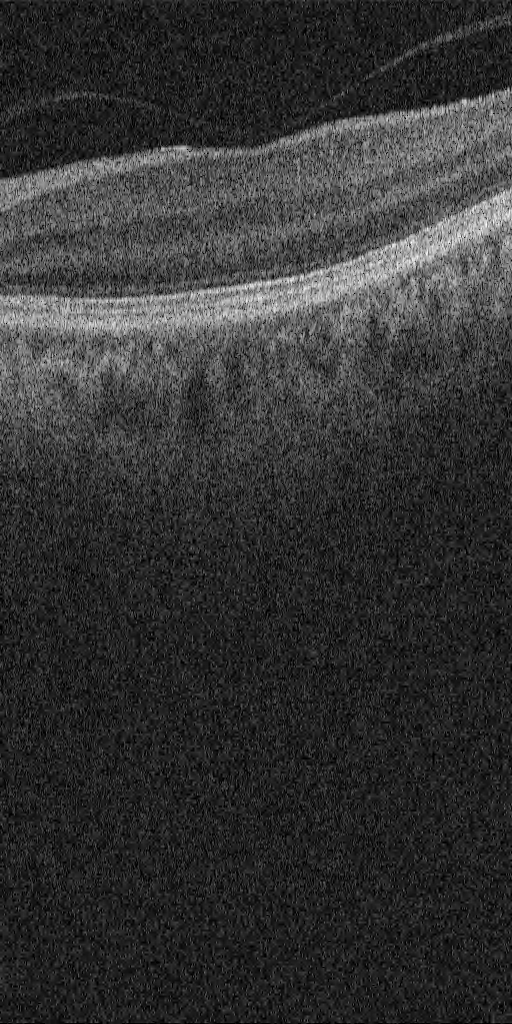
\includegraphics[scale=0.15]{normal_case.png}}\hfill
\subfigure[\ac{dme}-cyst]{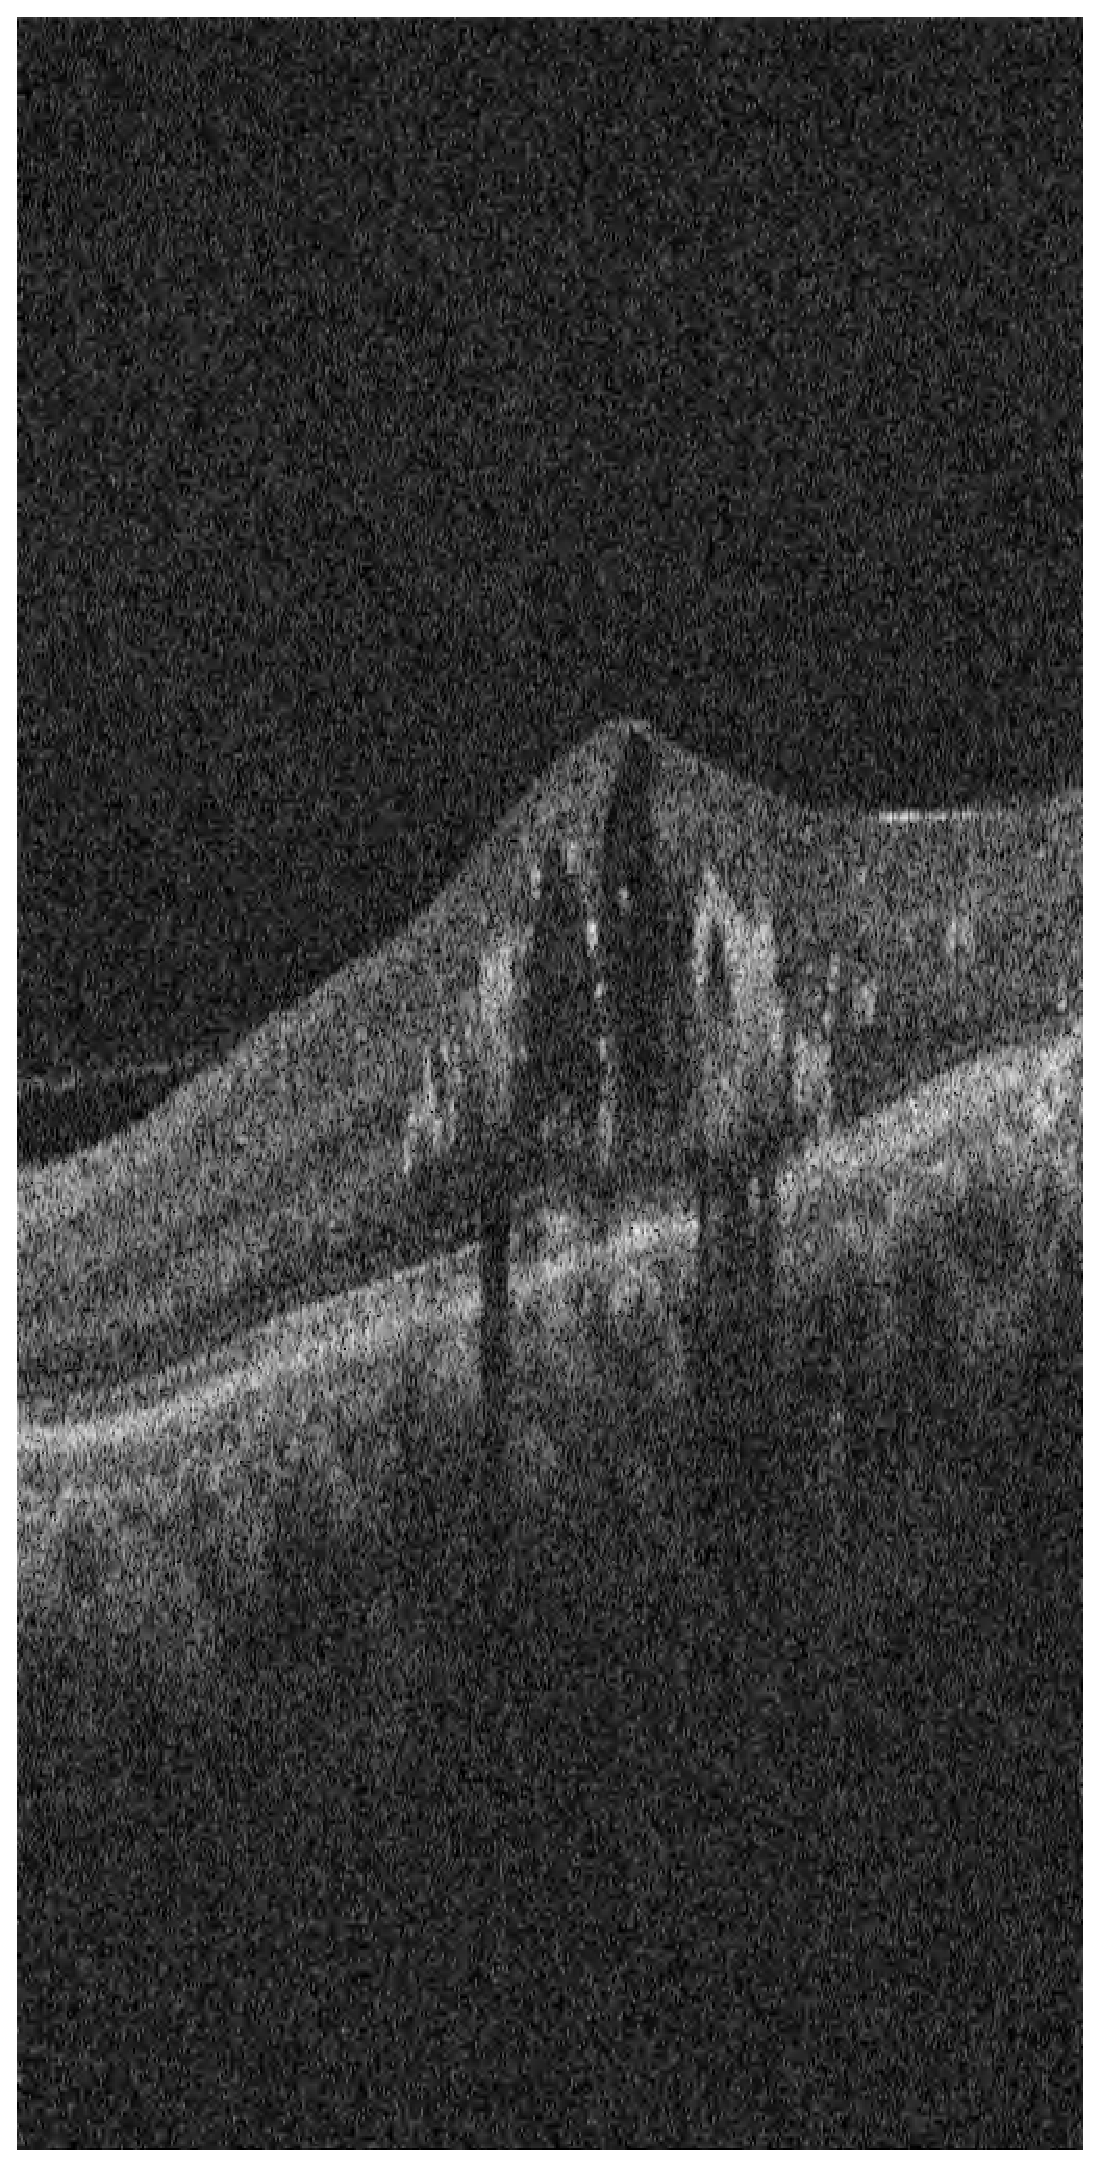
\includegraphics[scale=0.15]{dme_cyst}}\hfill
\subfigure[\ac{dme}-exudate]{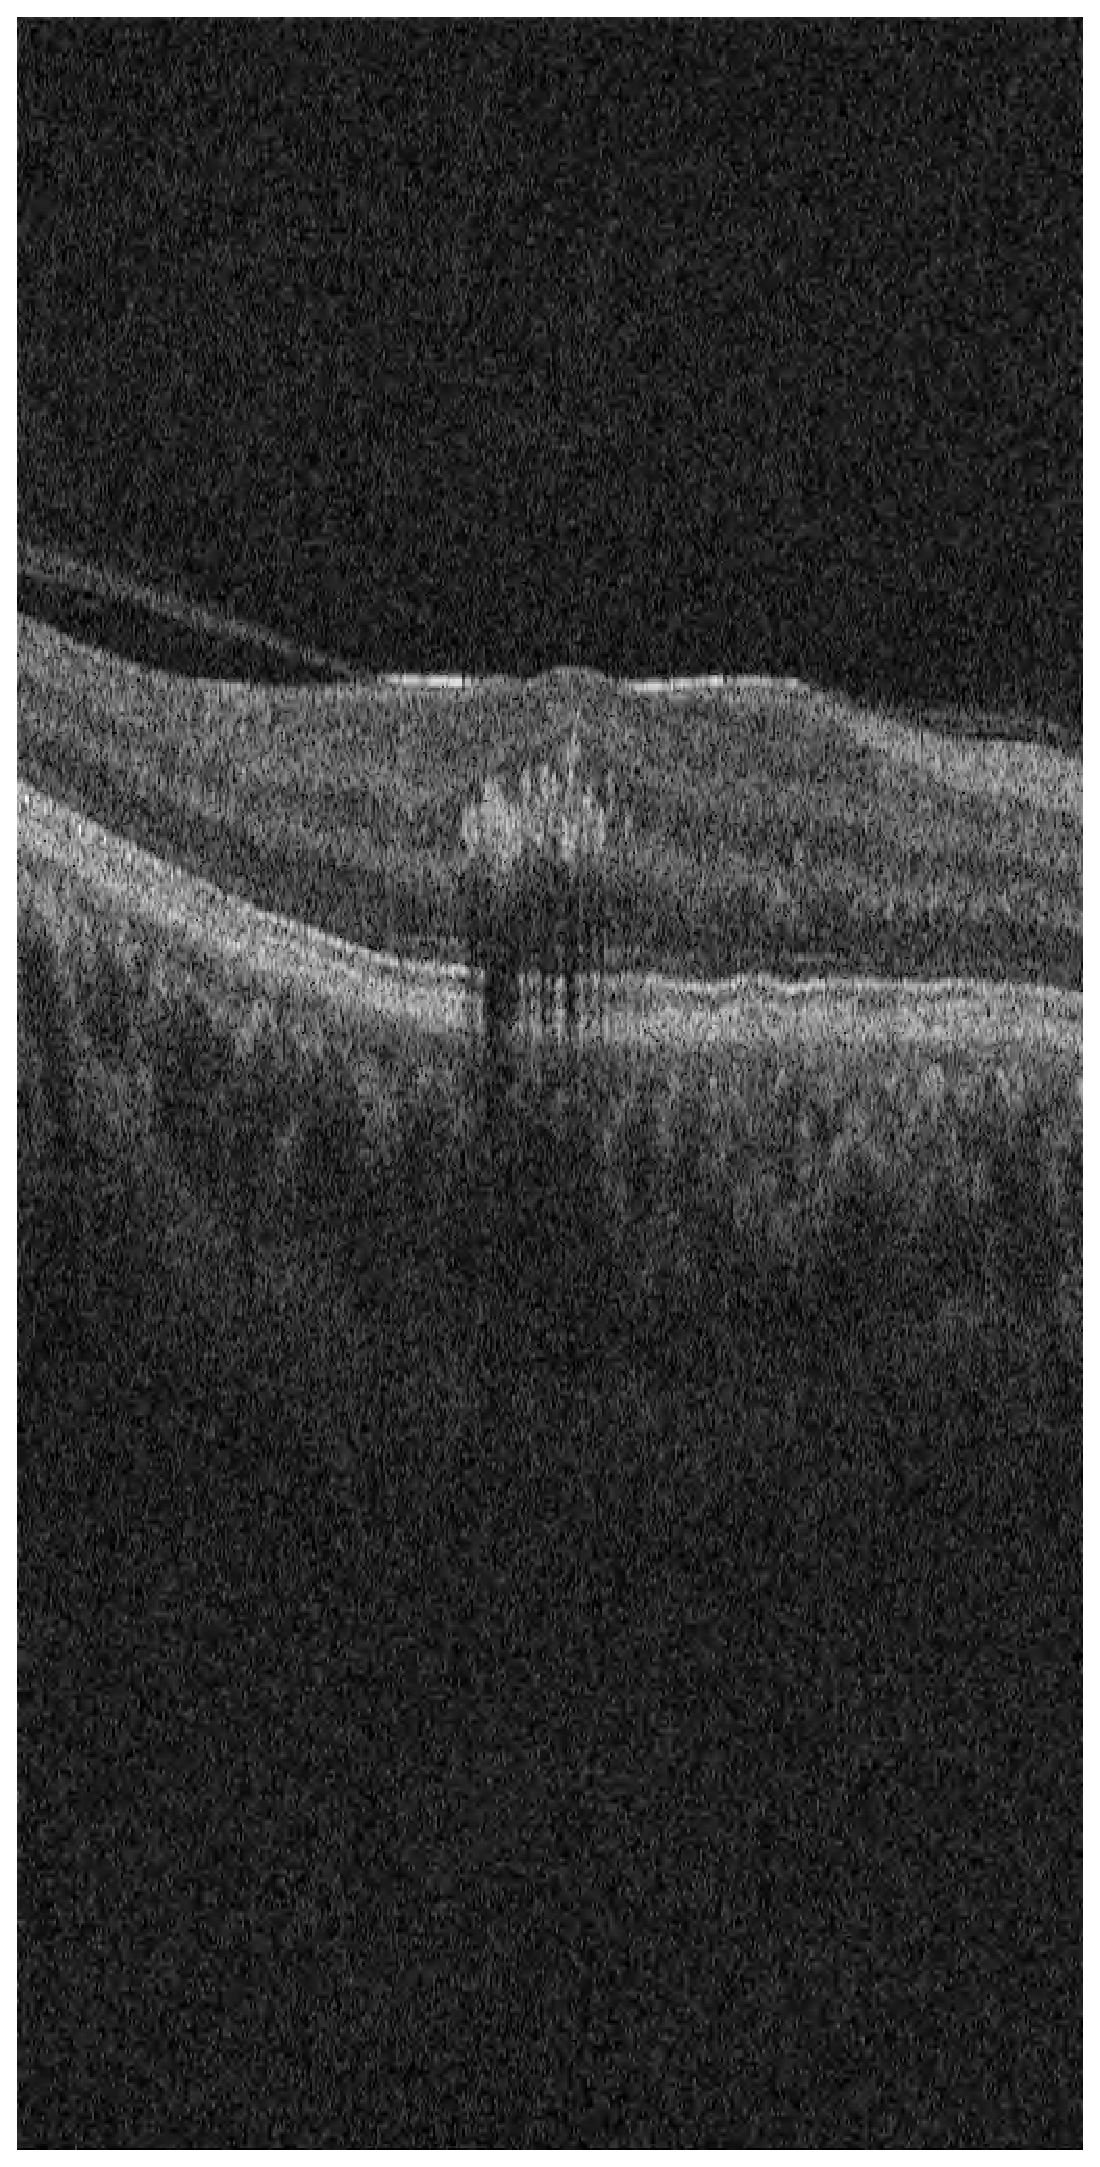
\includegraphics[scale=0.15]{dme_exudate}}
\hspace*{\fill}
\end{center}
\caption{ Example of \ac{sdoct} images for normal (a) and \ac{dme} patients (b)-(c) with cyst and exudate, respectively.}
\label{fig:dme-normal}
\end{figure}

Many of the previous works on \ac{oct} image analysis have focused on the problem of retinal layers segmentation, which is a necessary step for retinal
thickness measurements~\cite{Chiu2010,Kafieh2013}.
However, few have addressed the specific problem of \ac{dme} and its associated features detection from \ac{oct} images.

In this research we focus on the latter problem and propose an automatic framework for identification of \ac{dme} patients versus normal subjects using \ac{oct} volumes.
The proposed method, which is an extension of our previous work \cite{Lemaintre2015miccaiOCT}, is based on \ac{lbp} features to describe the texture of \ac{oct} images and dictionary learning using the \ac{bow} models~\cite{Sivic2003}.
We propose to extract 2D and 3D \ac{lbp} features from \ac{oct} images and volumes, respectively.
The \ac{lbp} descriptors are further extracted from the entire sample or local patches within individual samples.
In this research beside the comparison of 2D and 3D features, we also compare the effects of common pre-processing steps for \ac{oct} data, study the optimal configuration regarding the \ac{bow} approach in conjunction with different base classifiers.

%In the following of this paper, first in Sect.\,\ref{sec:rw} a summary of the related studies is presented.

This paper is organized as follows, Section~\ref{sec:rw} presents a summary of the related studies.
The proposed framework is explained in Sect.\,\ref{sec:method}, while the experiments and results are discussed in Sect.\,\ref{sec:exp}.
Finally, the conclusion and avenue for future directions are drawn in Sect.\,\ref{sec:con}.


%----------

%%% Local Variables:
%%% TeX-master: "../../main.tex"
%%% TeX-master: "../../main.tex"
%%% End:
          % the file wihtout .tex
% include the figures path relative to the master file
% \graphicspath{ {./content/survey/figures/} }

\section{Background}\label{sec:rw}
This section reviews the works straightly addressing the problem of classifying \oct volumes as normal or abnormal. A summary can be found in \Cref{tab:survey}.
%This section reviews, up to our knowledge, the works straightly addressing the problem of classifying \oct volume as normal or abnormal. A summary can be found in \Cref{tab:survey}.

Srinivasan\,\textit{et al.}~\cite{Srinivasan2014} proposed a classification method to distinguish \ac{dme}, \ac{amd} and normal \ac{sdoct} volumes.
%The authors in~\cite{Srinivasan2014} proposed a classification method for the detection of \ac{dme} versus \ac{amd} and normal \ac{oct} images.
The \ac{oct} images are pre-processed by reducing the speckle noise by enhancing the sparsity in a transform-domain and flattening the retinal curvature to reduce the inter-patient variations.
%The method is based on pre-processing to reduce the speckle noise in \ac{oct} images and flattening of the images to reduce the variation of retinal curvature among patients.
Then, \ac{hog} are extracted for each slice of a volume and a linear \ac{svm} is used for classification.
On a dataset of 45 patients equally subdivided into the three aforementioned classes, this method leads to a correct classification rate of $100 \%$, $100 \%$ and $86.67 \%$ for normal, \ac{dme} and \ac{amd} patients, respectively.
%On a dataset of 45 patients containing 15 normal subjects, 15 \ac{dme} patients and 15 \ac{amd} patients, the methods achieved a correct classification of $100 \%$, $100 \%$ and $86.67 \%$ for \ac{amd}, \ac{dme} and normal cases respectively.

Venhuizen\,\textit{et al.} proposed a method for \ac{oct} images classification using the \ac{bow} models~\cite{Venhuizen2015}.
The method starts with the detection and selection of keypoints in each individual B-scan, by keeping the most salient points corresponding to the top $3 \%$ of the vertical gradient values. Then, a texton of size $9 \times 9$ pixels is extracted around each keypoint, and \ac{pca} is applied to reduce the dimension of every texton to get a feature vector of size $9$.
All extracted feature vectors are used to create a codebook using \textit{k}-means clustering.
Then, the obtained codebook from the training is used to represent each \ac{oct} volume as a feature {\color{red}vector occurrence histogram}.
Finally, this histogram is used as feature vector to train a \ac{rf} with a maximum of $100$ trees.
The method was used to classify \ac{oct} volumes between \ac{amd} and normal cases and achieved an \ac{auc} of $0.984$ with a dataset of $384$ \ac{oct} volumes.

Liu\,\textit{et al.} proposed a methodology for detecting macular pathology in \ac{oct} images using \ac{lbp} and gradient information as attributes~\cite{Liu2011}.
The method starts by aligning and flattening the images and creating a $3$-level multi-scale spatial pyramid.
The edge and \ac{lbp} histograms are then extracted from each block of every level of the pyramid.
%is created and edge and \ac{lbp} histograms are extracted in each block at every level of the pyramid.
All the obtained histograms are concatenated into a global descriptor whose dimensions are reduced using \ac{pca}.
Finally a \ac{svm} is used as classifier.
The method achieved good results in detection \ac{oct} scan containing different pathology such as \ac{dme} or \ac{amd}, with an \ac{auc} of $0.93$ using a dataset of $326$ \ac{oct} scans.

{\color{red} In our later study, }\added[id= sik]{Lema\^itre\,\textit{et al.} proposed a standard classification procedure to differentiate between \ac{dme} and normal \ac{sdoct} volumes.
The data is pre-processed using \ac{nlm} filtering.
The volumes are mapped into discrete set of structures namely local when these structures correspond to patches, or global when the structures correspond to volume slices or the whole volume.
These structures are described in terms of \ac{lbp}, or \ac{lbp} from \ac{lbptop}, and when necessary to represent each volume as a single feature vector, these structures are encoded either using histogram, \ac{pca} or \ac{bow}, to present the volumes to a \ac{rf} classifeir.
This methodology was tested against Venhuizen\,\textit{et al.}~\cite{Venhuizen2015} using public and non-public datasets showing an improvement within the results achieving a \ac{se} of 87.5\% and a \ac{sp} of 100\%.}

\added[id = moj]{In our latest study~\cite{Lemaintre2015miccaiOCT}, we proposed a classification framework for differentiating \ac{dme} and normal \ac{sdoct} volumes.
In this work, we proposed to pre-process the volumes using \ac{nlm} filtering and mapped them either into a set of structures, corresponding to patches from slices or volumes (local) or a single structure per slice or volume (global).
From the considered structures we proposed to extract \ac{lbp} and \ac{lbptop} features and represent them using histogram, \ac{pca} or \ac{bow} algorithm.
The represented features were then classified using \ac{rf} classifier.
This methodology was tested on public and non-public dataset and the obtained results revealed improvement against Venhuizen\,\textit{et al.}~\cite{Venhuizen2015} algorithm by achieving the \ac{se} and \ac{sp} of 87.5\% and 100\%, respectively.
The obtained results from this study is listed in Sect.\,\ref{sec:exp}.
As stated in previous section, this research is a continue of our previous work, where we intend to evaluate the influence of different pre-processing, \ac{bow} representation and various classifiers.
Our proposed pipeline with detail description of each step is presented in the following section
 }
%\DTLloaddb[keys={task,Srinivasan,Venhuizen,Liu,Lemaitre}]
%          {survey}{./content/survey/tables/survey.csv}
%\begin{table}
%  \caption{Other methodologies overview}
%  \centering
%  \documentclass[%
  border=1pt
  % border={0pt 20pt 0pt 0pt} % left bottom right top
]{standalone}% http://ctan.org/pkg/standalone

% Stuff defined here is not loaded at the parent document
%
\usepackage{datatool}
\usepackage{booktabs}
\usepackage{subfigure}

\DTLloaddb[keys={task,Srinivasan,Venhuizen,Liu,Lemaitre}]{survey}{survey.csv}
task,srinivasan,venhuizen,liu,lemaintre
\begin{document}
  \begin{tabular} {ccccc}
    \toprule
    &
    \textbf{Srinivasan\,\textit{et al.}~\cite{Srinivasan2014}} &
    \textbf{Venhuizen\,\textit{et al.}~\cite{Venhuizen2015}} &
    \textbf{Liu\,\textit{et al.}~\cite{Liu2011}} &
    \textbf{Lema{\^i}ntre\,\textit{et al.}~\cite{Lemaintre2015miccaiOCT}} \\

    \DTLforeach{survey}{\task=task,\srini=Srinivasan,\venhu=Venhuizen,
                        \liu=Liu, \lemaitre=Lemaitre}{%
    \\ \task & \srini & \venhu & \liu & \lemaitre}
  \end{tabular}
\end{document}

%  \label{tab:survey}
%\end{table}


\begin{landscape}
\begin{table}
\caption{The summary of the state of the art methods}
\resizebox{1\linewidth}{!}{
\scriptsize{
\begin{tabular}{l ccc c cccc	c c ccc}
\toprule
Ref & \multicolumn{3}{c}{Task} & Data size & \multicolumn{4}{c}{Pre-processing} & features & Classifier & \multicolumn{3}{c}{Evaluation}\\
\cmidrule(l){2-4}\cmidrule(l){6-9} \cmidrule(l){12-14}
    & \ac{amd} & \ac{dme} & normal     &           & de-noise & Flatten & aligned & Cropped &   &  & \ac{se} & \ac{sp} & \ac{auc}\\
\midrule
& & & & & & & & & & & & &  \\

Srinivansan\,\textit{et al.}~\cite{Srinivasan2014} & $\checkmark$ & $\checkmark$ & $\checkmark$ &  45 & $\checkmark$ & $\checkmark$ &  & $\checkmark$ & \ac{hog} & \ac{svm} & 86.7\%,100\%,100\% & &  \\
& & & & & & & & & & & & &    \\

Venhuizen\,\textit{et al.}~\cite{Venhuizen2015} & $\checkmark$ &  & $\checkmark$ & 384 &  & & & &  texton  & \acs{rf} & & & 0.984 \\ 
& & & & & & & & & & & & &   \\

Liu\,\textit{et al.}~\cite{Liu2011} & $\checkmark$ & $\checkmark$ & $\checkmark$  & 326 &  & $\checkmark$ & $\checkmark$ &  &  Edge, \ac{lbp} & \acs{svm} & & &  0.93 \\
& & & & & & & & & & & & &   \\

Lema\^itre\,\textit{et al.}~\cite{Lemaintre2015miccaiOCT} &  & $\checkmark$ & $\checkmark$ & 32  & $\checkmark$ &  &  &  & \acs{lbp}-\acs{lbptop} & \ac{rf} & 87.5\% & 75\% & \\
& & & & & & & & & & & & &   \\
\bottomrule
\end{tabular}}}
\label{tab:survey-tab}
\end{table}

\begin{figure}
  \centering{
    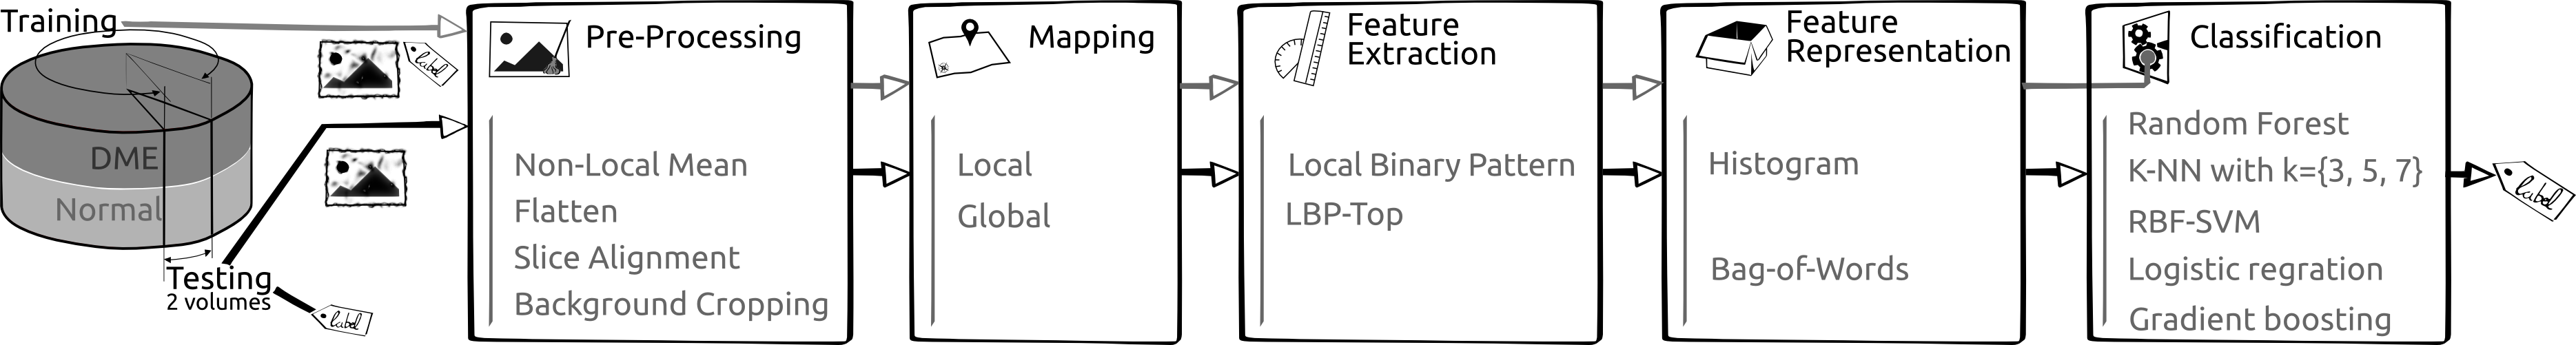
\includegraphics[width=1\linewidth]{content/survey/ml.png}}
  \caption{Machine learning classification basic scheme}
  \label{fig:ML-scheme}
\end{figure}



\end{landscape}
    % the file wihtout .tex
% include the figures path relative to the master file
% \graphicspath{ {./content/method/figures/visual_cues/}{./content/method/figures/}}
\graphicspath{ {./content/method/figures/}}

\section{Materials and Methods}\label{sec:method}
%\todo{Mention texture here, rework where the sections are called}

The proposed method, as well as, its experimental set-up for \ac{oct} volume classification are outlined in Fig.\,\ref{fig:ML-scheme}.
%The methodology is formulated as a standard classification procedure.
The methodology is formulated as a standard classification procedure which consists of five steps.
First, the \ac{oct} volumes are pre-processed as presented in details in Sect.\,\ref{subsec:prepro}.
%Then toward a final descriptor \ac{lbp} and \ac{lbptop} features are extracted with different mapping strategy and represented using two approach.
Then, \ac{lbp} and \ac{lbptop} features are detected, mapped and extracted as discussed in depth in Sect.\,\ref{subsec:feaext}, Sect.\,\ref{subsec:mapping}, and Sect.\,\ref{subsec:fearep}, respectively.
%{\color{red}The feature extraction, mapping, and representation are presented in depth in Sect.\,\ref{subsec:feaext}, Sect.\,\ref{subsec:mapping}, and Sect.\,\ref{subsec:fearep}, respectively. CHECK THE SECTION ORDERING}
Finally, the classification step is presented in Sect.\,\ref{subsec:cls}.


\subsection{Image pre-processing}\label{subsec:prepro}

This section describes the set of pre-processing techniques which aim at enhancing the \ac{oct} volume.
The influence of these pre-processing methods and their possible combinations are extensively studied in Sect.\,\ref{subsec:exp2}-\ref{subsec:exp4}.

\subsubsection{\acf{nlm}}

\begin{figure}[t]
  \centering
  \hspace*{\fill}
  \subfigure[]{\label{subfig:vol}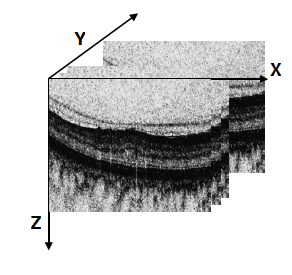
\includegraphics[width=0.3\linewidth]{axs.png}} \hfill
  \subfigure[]{\label{subfig:raw}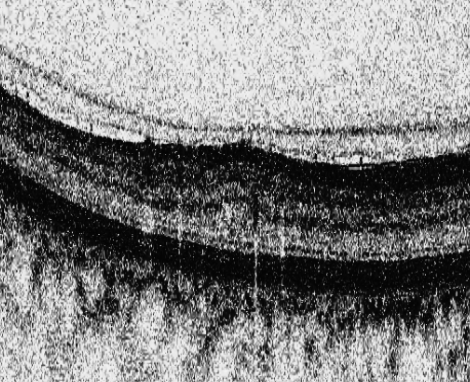
\includegraphics[width=0.3\linewidth]{raw_crop_grey.png}} \hfill
  \subfigure[]{\label{subfig:nlm}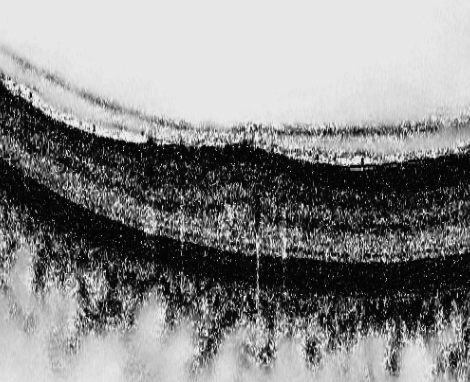
\includegraphics[width=0.3\linewidth]{nlm_crop_grey.png}}
  \hspace*{\fill}
  \caption{\ac{oct}: (a) Organization of the \ac{oct} data - (b) Original image - (c) \ac{nlm} filtering. Note that the images have been negated for visualization purposes.}
  \label{fig:denoise}
\end{figure}


\ac{oct} images suffer from speckle noise, like other image modalities such as \ac{us}~\cite{schmitt1999speckle}.
The \ac{oct} volumes are enhanced by denoising each B-scan (i.e. each $x-z$ slice) using the \ac{nlm}~\cite{buades2005non}, as shown in Fig.\,\ref{fig:denoise}.
\ac{nlm} has been successfully applied to \ac{us} images to reduce speckle noise and outperforms other common denoising methods~\cite{Coupe2009}.
\ac{nlm} filtering preserves fine structures as well as flat zones, by using all the possible self-predictions that the image can provide rather than local or frequency filters such as Gaussian, anisotropic, or Wiener filters~\cite{buades2005non}.
%An example of filtering using \ac{nlm} filter on \ac{oct} image is depicted in Fig\,\ref{subfig:raw} and Fig.\,\ref{subfig:nlm}.

\subsubsection{Flattening}


\begin{figure}[t]
\centering 
  \hspace*{\fill}
  \subfigure[]{\label{subfig:flatorg}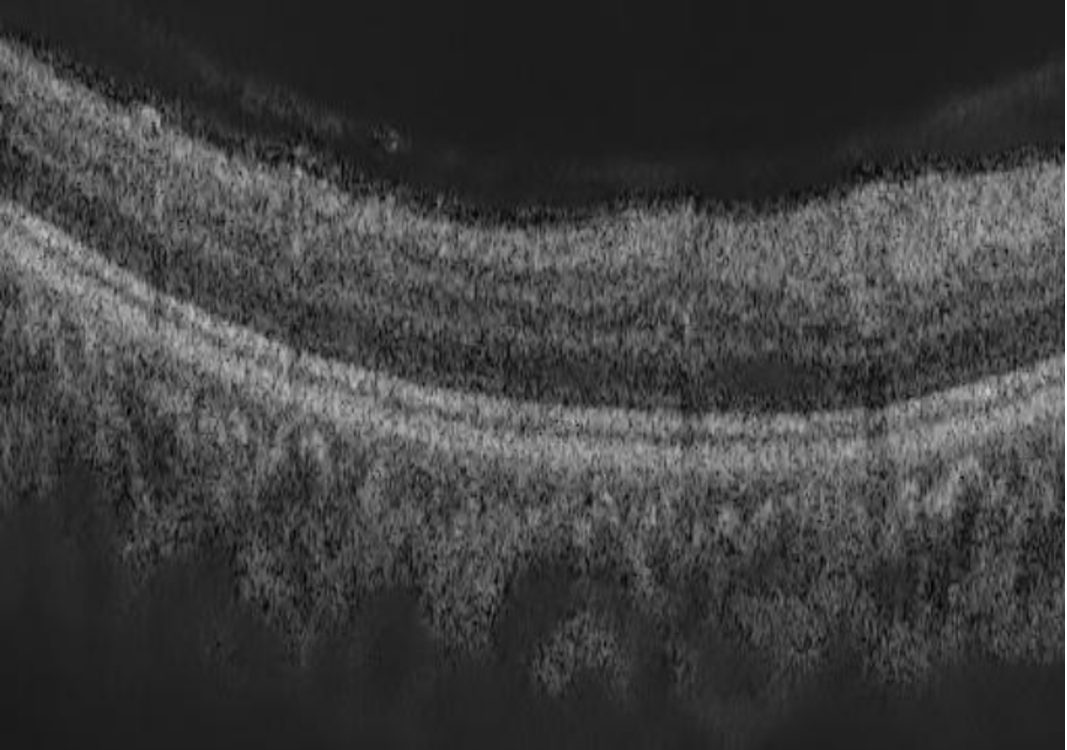
\includegraphics[width=0.20\textwidth]{flattening/original_cropped}}\hfill
  \subfigure[]{\label{subfig:flatotsu}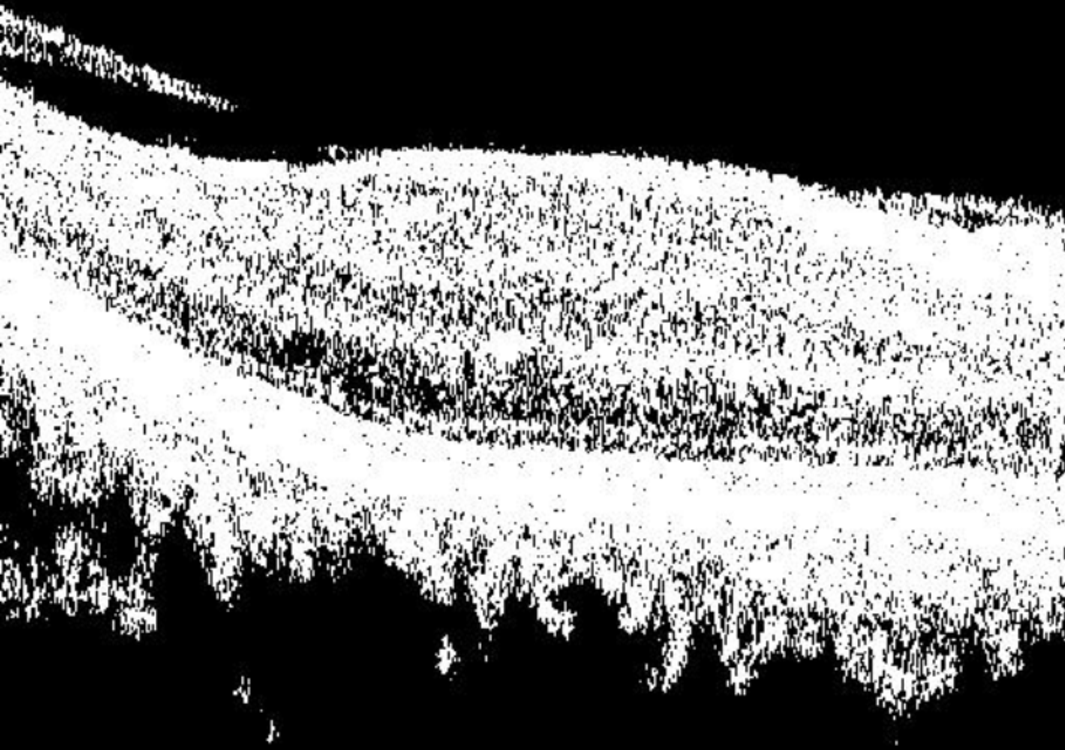
\includegraphics[width=0.20\textwidth]{flattening/thresholding_cropped}}\hfill
  \subfigure[]{\label{subfig:flatmedian}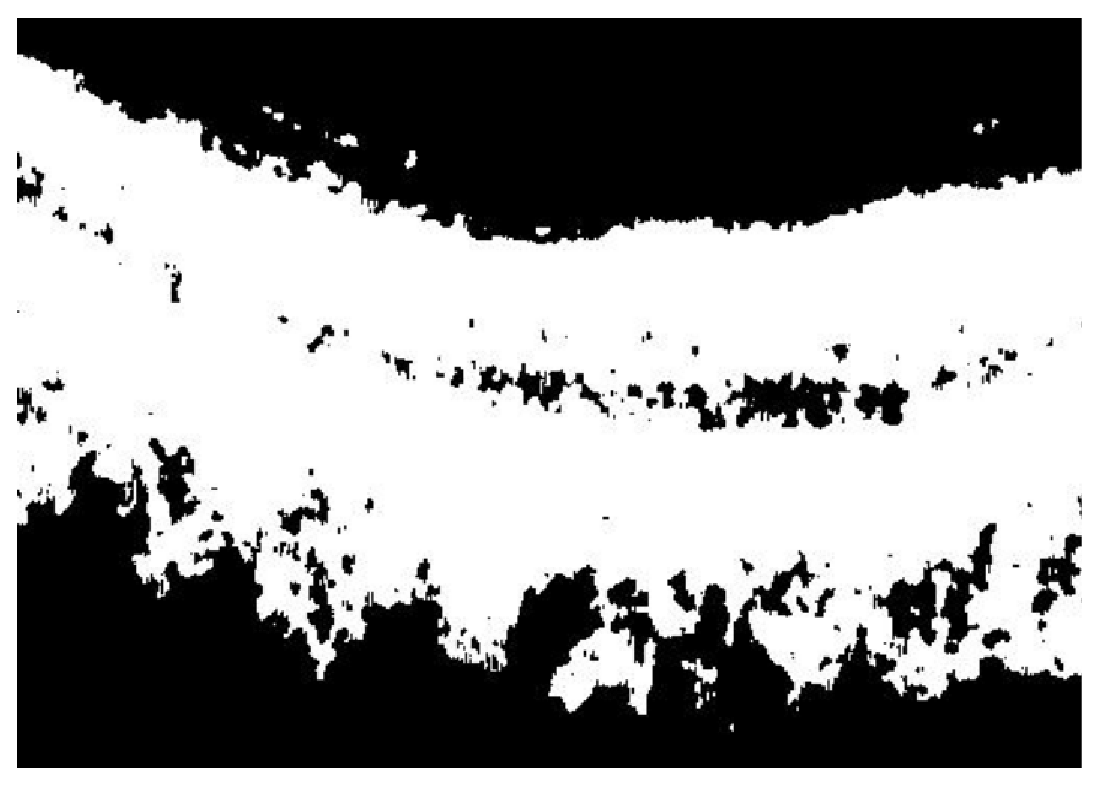
\includegraphics[width=0.20\textwidth]{flattening/median_cropped}}
  \hspace*{\fill}	
  \\
  \hspace*{\fill}
  \subfigure[]{\label{subfig:flatfit}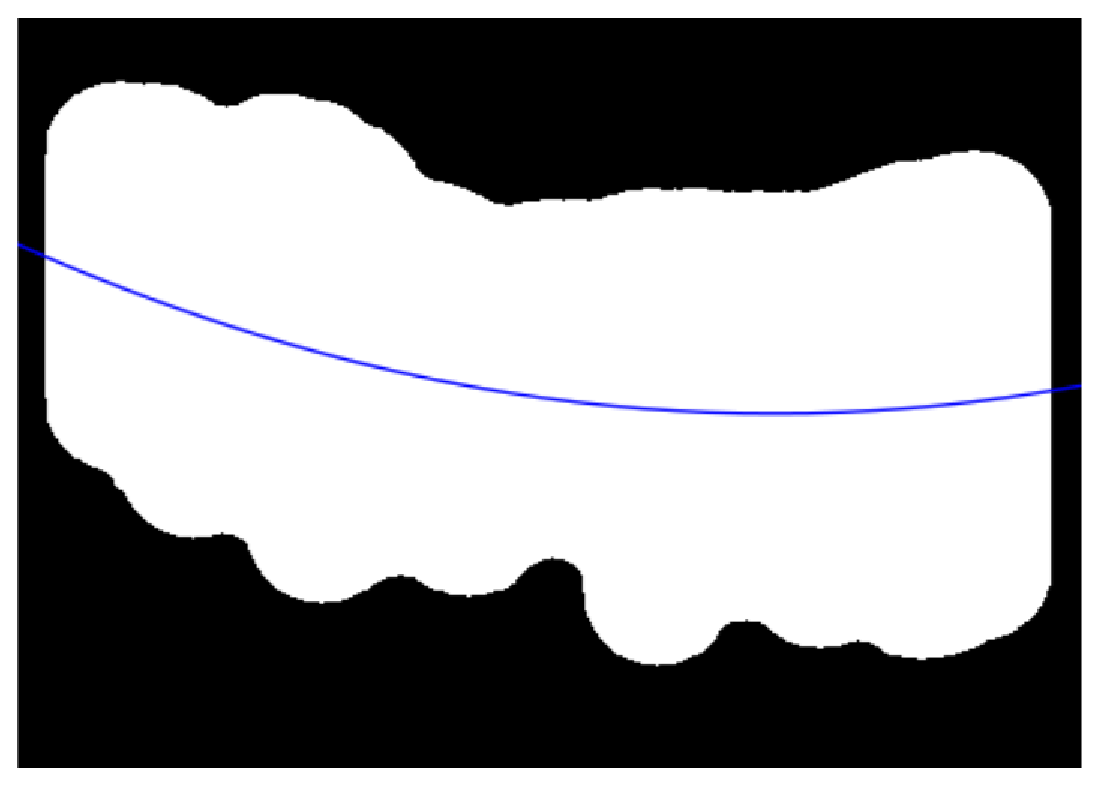
\includegraphics[width=0.20\textwidth]{flattening/fit_cropped}}\hfill
  \subfigure[]{\label{subfig:flatwarp}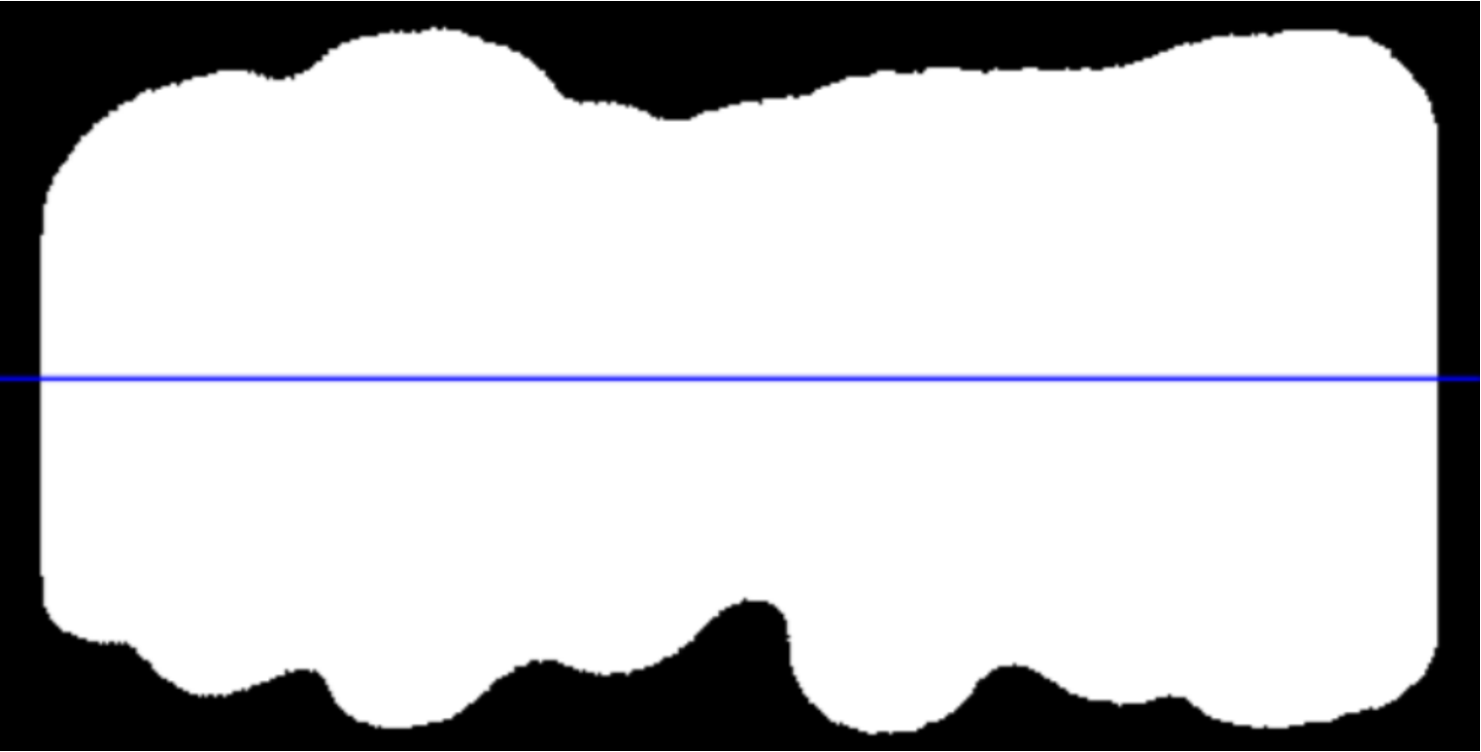
\includegraphics[width=0.20\textwidth]{flattening/warped_cropped}}\hfill
  \subfigure[]{\label{subfig:flatfinal}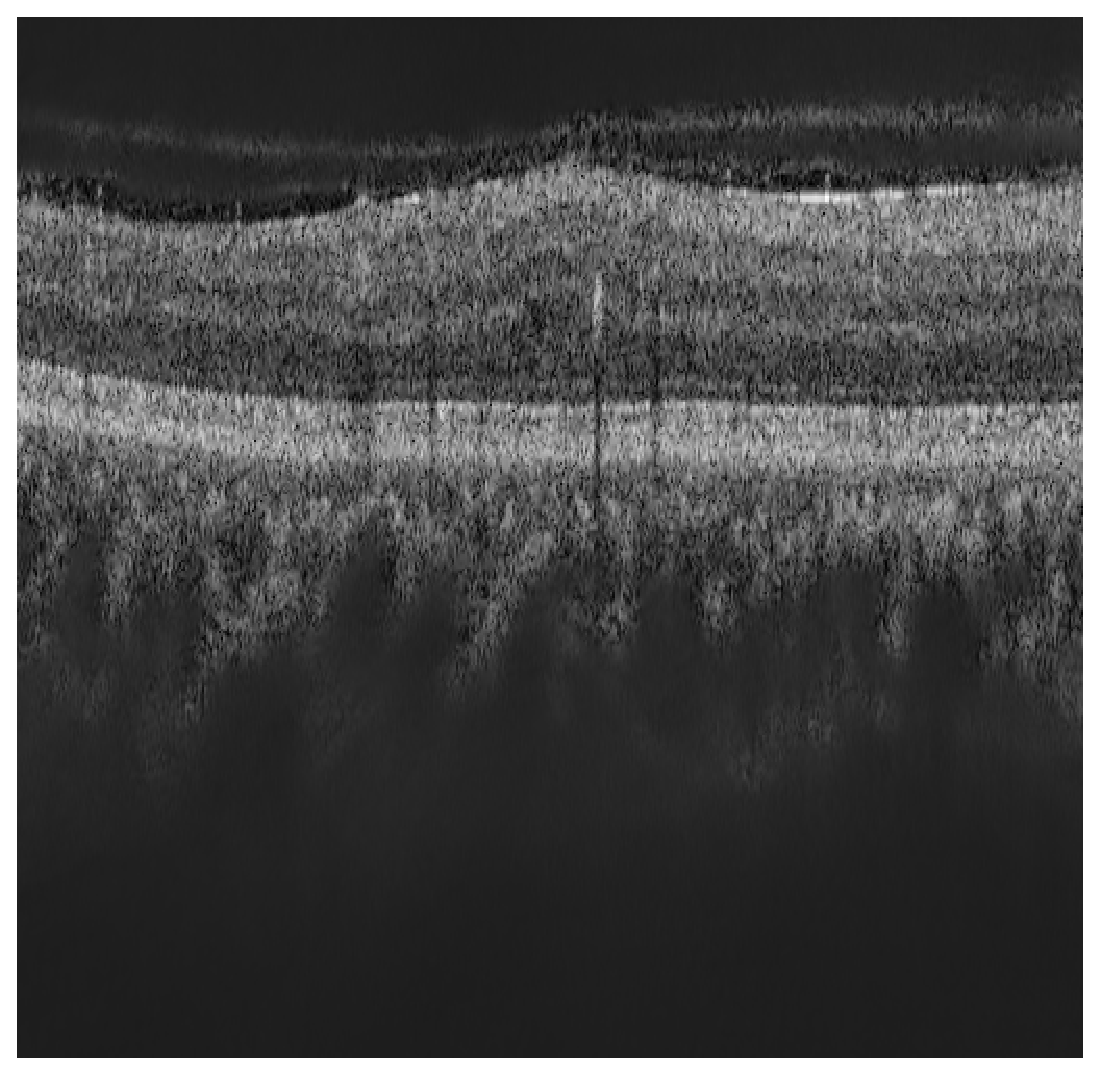
\includegraphics[width=0.20\textwidth]{flattening/warped_org_cropped}}
  \hspace*{\fill}
  \caption{Flattening procedure: (a) original image, (b) thresholding, (c) median filtering, (d) curve fitting, (e) warping, (f) flatten image.}
  \label{fig:flatten}
\end{figure}

Textural descriptors characterize spatial arrangement of intensities.
However, the \ac{oct} scans suffer from large type of variations: inclination angles, positioning, and natural curvature of the retina~\cite{Liu2011}.
Therefore, these variations have to be taken into account to ensure a consistent characterization of the tissue disposition, regardless of the location in the retina.
This invariance can be achieved from different manners: (i) using a rotation invariant descriptor (cf. Sect.\,\ref{subsec:feaext}), or (ii) by unfolding the curvature of the retina.
This latter correction is known as image flattening which theoretically consists of two distinct steps: (i) estimate and fit the curvature of the \ac{rpe} and (ii) warp the \ac{oct} volume such that the \ac{rpe} becomes flat.

Our correction is similar to the one of Liu\,\textit{et al.}~\cite{Liu2011}: each B-scan is thresholded using Otsu's method followed by a median filtering to detect the different retina layers (see Fig\,\ref{subfig:flatmedian} and Fig\,\ref{subfig:flatotsu}). 
Then, a morphological closing and opening is applied to fill the holes and the resulting area is fitted using a second-order polynomial (see Fig.\,\ref{subfig:flatfit}). 
Finally, the scan is warped such that the curve becomes a line as presented in Fig.\,\ref{subfig:flatwarp} and Fig.\,\ref{subfig:flatfinal}. 

%This process of unfolding the curvature of the retina is known as image flattening. When flattening, an estimation of the \rpe  layer is used to modify the volume by imposing that the \rpe  should be flat.
%Our implementation modifies the proposal of Liu\,\textit{et al.}~\cite{Liu2011}, as illustrated in \Cref{fig:flatten}. Othsu thresholding is used to segment the retina from the background. A line is fitted to the bottom part of the segmentation hull, since it is assumed to be parallel to the \rpe. The image is corrected based on this line.

\subsubsection{Slice alignment}
The flattening correction does not enforce an alignment through the \ac{oct} volume.
Thus, in addition to the flattening correction, the warped curves of each B-scan are positioned at the same altitude in the $z$ axis. 

%Similarly, when using 3D texture, misalignment between the slice introduce error to the texture descriptor. In this case the slices are also aligned based on the segmentation's hull.

%\subsubsection{Background cropping}
%\todo[inline]{Cropping out the background allows for less texture to be encoded}

\subsection{Feature detection}\label{subsec:feaext}
In this research, we choose to detect simple and efficient \ac{lbp} texture features with regards to each \ac{oct} slice and volume.
\ac{lbp} is a texture descriptor based on the signs of the differences of a central pixel with respect to its neighboring pixels~\cite{ojala2002multiresolution}.
These differences are encoded in terms of binary patterns as in~Eq.\,\eqref{Eq:LBP}:

\begin{equation}\label{Eq:LBP}
LBP_{P,R} = \sum_{p=0}^{P-1}s(g_{p} - g_{c})2^{p} \ , \qquad s(x) = \begin{cases}
    1  & \ \text{if } x \geq 0\\
    0  & \ \text{otherwise}\\
  \end{cases} \ ,
\end{equation}

\noindent where $g_c$, $g_{p}$ are the intensities of the central pixel and a given neighbor pixel, respectively. $P$ is the number of sampling points in the circle of radius $R$.
Ojala\,\textit{et al.} further extended the original \ac{lbp} formulation to achieve rotation invariance at the expense of limiting the texture description to the notion of circular ``uniformity''~\cite{ojala2002multiresolution}.
Volume encoding is later proposed by Zhao\,\textit{et al.} by computing \ac{lbp} descriptors in three orthogonal planes, so called \ac{lbptop}~\cite{zhao2012rotation}.

In this research, we consider rotation invariant and uniform \ac{lbp} and \ac{lbptop} features with various sampling points (i.e., $\{8,16,24\}$) with respect to different radius, (i.e., $\{1,2,3\}$).
The number of patterns ($LBP_{\#pat}$) in regards with each configuration is reported in Table~\ref{tab:lbphist}.

%Table.~\ref{tab:lbphist} shows the length of uniform rotation invariant histogram ($\ac{lbp}_{hist}$) for the used sampling point and radius.
\begin{table}
\caption{Number of patterns ($LBP_{\#pat}$) for different sampling points and radius ($\{P,R\}$) of the \ac{lbp} descriptor.}
\centering{
\resizebox{0.5\linewidth}{!}{
\footnotesize{
\begin{tabular}{l  c c c }
\toprule
 \multicolumn{4}{c}{Sampling point for a radius ($\{P, R\}$)}\\
 \midrule
 & $\{8, 1\}$ & $\{16, 2\}$ & $\{24, 3\}$\\
 \cmidrule{2-4}
  $LBP_{\#pat}$  & 10 & 18 & 26 \\
 \bottomrule
\end{tabular}}}}
\label{tab:lbphist}
\end{table}
%\begin{figure}[t]
%  \centering
%  \hspace*{\fill}
%  \subfigure[]{\label{subfig:lbp}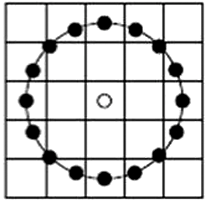
\includegraphics[height=0.1\textheight]{lbp.png}} \hfill
%  \subfigure[]{\label{subfig:lbptop}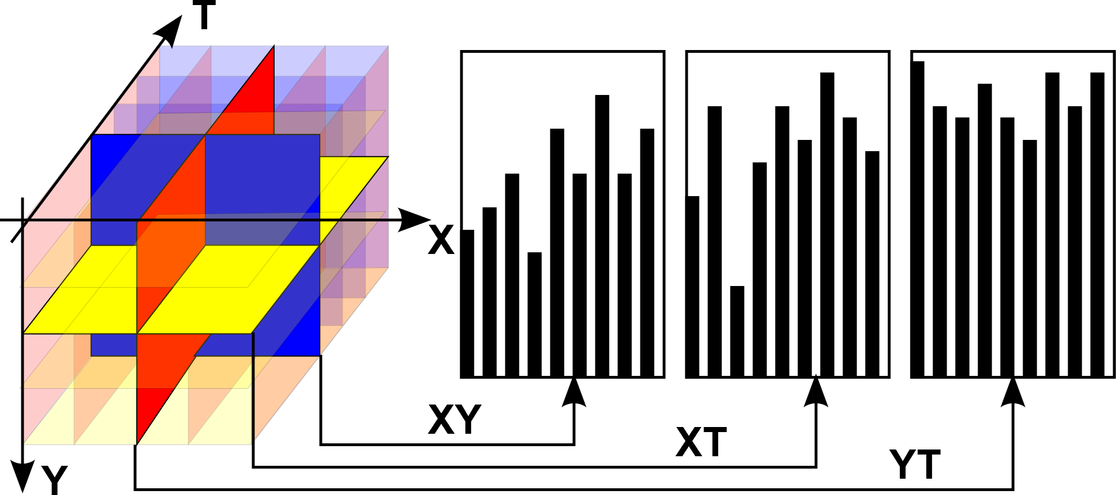
\includegraphics[height=0.1\textheight]{LBPTOP_fig.png}}
%  \hspace*{\fill}
%  \caption{The different \ac{lbp} descriptors: (a) \ac{lbp} with $(R=2,P=16)$ - (b) \ac{lbptop}~\cite{zhao2012rotation}.}
%  \label{fig:lbp}
%\end{figure}

\subsection{Mapping} \label{subsec:mapping}
The mapping stage is used to partition the previously computed feature images to later extract the final descriptor as presented in the next section.
%The mapping stage is used to determine a discrete set of elements (or structures) which is used for representing the \ac{oct} volume.
For this work, two mapping strategies are defined: (i) \emph{global} and (ii) \emph{local} mapping.

\begin{figure}[t]
\begin{center}
\hspace*{\fill}
\subfigure[]{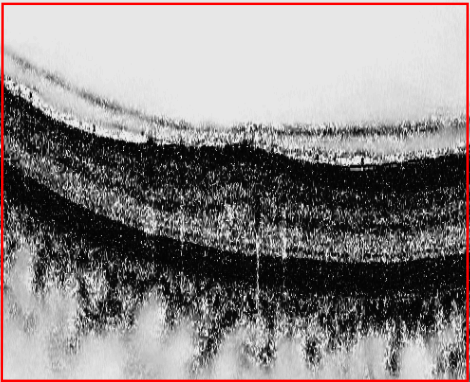
\includegraphics[width=0.22\textwidth]{/mapping/global-2d.png}\label{fig:gm1}}\hfill
\subfigure[]{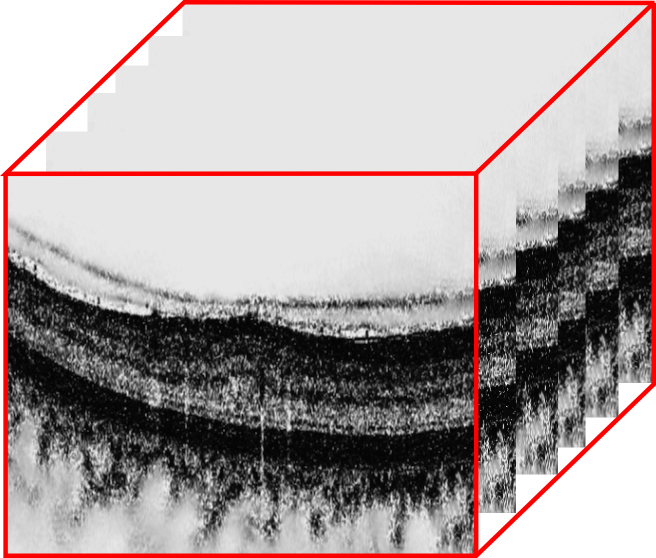
\includegraphics[width=0.22\textwidth]{/mapping/global-3d.png}\label{fig:gm2}}\hfill
\subfigure[]{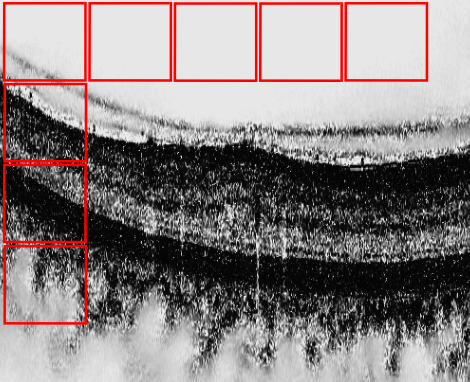
\includegraphics[width=0.22\textwidth]{/mapping/local-2d.png}\label{fig:lm1}}\hfill
\subfigure[]{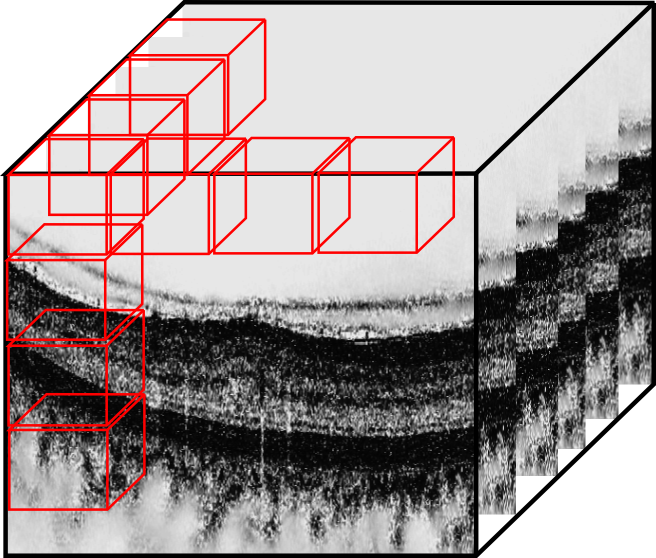
\includegraphics[width=0.22\textwidth]{/mapping/local-3d.png}\label{fig:lm2}}
\hspace*{\fill}
\caption{\emph{Global} (a)-(b) and \emph{local} (c)-(d) mapping for \ac{lbp} and \ac{lbptop} features (2D B-scan and 3D volume, respectively).}
\end{center}
\label{fig:lgmapping}
\end{figure}

\begin{description}
\item[\emph{Global}] mapping considers to extract the final descriptors from the 2D feature image for \ac{lbp} and 3D volume for \ac{lbptop}.
%mapping considers to extract the features from the 2D B-scans for \ac{lbp} and 3D volume for \ac{lbptop}.
Therefore, for a volume with $d$ slices, the \emph{global}-\ac{lbp} mapping will lead to the extraction of $d$ elements.
While the \emph{global}-\ac{lbptop} represents the whole volume as a single element.
The \emph{global} mapping for 2D images and 3D volume is shown in Fig.~\ref{fig:gm1} and \ref{fig:gm2}.

\item[\emph{Local}] mapping considers to extract the final descriptors from a set of ($m \times m$) 2D patches for \ac{lbp} and a set of ($ m \times m \times m$) sub-volumes for \ac{lbptop}.
Given $N$ and $N'$ the total number of 2D patches and 3D sub-volumes respectively, the \emph{local}-\ac{lbp} approach provides $N \times d$ elements, while \emph{local}-\ac{lbptop} provides $N'$ elements.
%Here $N$ and $N'$ are the total number of elements per B-scane or the volume, respectively.
This mapping is illustrated in Fig.~\ref{fig:lm1} and \ref{fig:lm2}.


\end{description}

%For the sake of clarification, the length of final descriptor for \emph{local} and \emph{global} mapping of both \ac{lbp} and \ac{lbptop} features with respect to the length of $\ac{lbp}_{hist}$ are listed in Table.~\ref{tab:tabmap}.
%
%\begin{table}[h]
%\caption{ Final length of descriptors of \ac{lbp} and \ac{lbptop} features, with respect to different mapping strategies and $\ac{lbp}_{hist}$ number of bins for various sampling point. Here $d$ is the number of B-scans per volumes and $N$ and $N'$ are the number of patches per B-scane and sub-volumes per volumes, respectively.}
%\centering
%\resizebox{1\linewidth}{!}{
%\scriptsize{
%\begin{tabular}{l ccc c ccc }
%\toprule
%Mapping & \multicolumn{3}{c}{\ac{lbp}} & & \multicolumn{3}{c}{\ac{lbptop}}\\
%\cmidrule(l){2-4} \cmidrule(l){6-8}
% & $\{8,1\}$ & $\{16,2\}$ & $\{24,3\}$ &  & $\{8,1\}$ & $\{16,2\}$ & $\{24,3\}$\\ 
% \midrule
%\emph{global} & $10 \times d $ & $ 18 \times d $ & $26 \times d$ & &  $ 3 \times 10 $ & $ 3 \times 18 $ & $3 \times 26$  \\
% & & & & & & & \\
%\emph{local} & $10 \times N \times d$ & $18 \times N \times d$ & $26 \times N \times d$ & & $3 \times 10 \times N' \times \frac{m}{d}$ & $3 \times 18 \times N'\times \frac{m}{d} $ & $3 \times 26 \times N'\times \frac{m}{d}$     \\
%\bottomrule
%\end{tabular}}
%}
%\label{tab:tabmap}
%\end{table}


\subsection{Feature extraction}\label{subsec:fearep}

% Each \ac{oct} volume can be described by its texture and we employed two strategies.
Two strategies are used to describe each \ac{oct} volume texture.

\begin{description}

\item[Low-level representation] The texture descriptor of an \ac{oct} volume is defined as the concatenation of the \ac{lbp} histograms with the \emph{global}-mapping.
The \ac{lbp} histograms are extracted from the previously detected \ac{lbp} images (see Sect.\,\ref{subsec:feaext}).
Therefore, the \ac{lbptop} final descriptor is computed through the concatenation of the \ac{lbp} histograms of the three orthogonal planes with the final size of $3 \times LBP_{\#pat}$.
Similarly, the \ac{lbp} descriptor is defined through concatenation of the \ac{lbp} histograms per each slice with the final size of $d \times LBP_{\#pat}$.

\item[High-level representation] The concatenation of histograms employed in the low-level representation in conjunction with either \emph{global}- or \emph{local}-mapping can lead lead to a high dimensional feature space.
For instance, \emph{local}-mapping results to a size of $N \times d \times LBP_{\#path}$ for the final \ac{lbp} descriptor and $N' \times LBP_{\#path}$ for the final \ac{lbptop} descriptor.
High-level representation simplifies this high dimensional feature space into a more discriminant lower space.
\ac{bow} approach is used for this purpose~\cite{Sivic2003}.
This model represents the features by creating a codebook or visual dictionary, from the set of low-level features.
The set of low-level features are clustered using \textit{k}-means to create the codebook with \textit{k} clusters or visual words.
After creating the codebook, each of the training example is represented as a histogram of size \textit{k}.
The histogram is obtained by calculating the frequency of occurrences of each of the \textit{k} words in the extracted features from the training example.
%\Ac{pca} and \ac{bow} among other methods, are used for this purpose~\cite{Sivic2003}.
%Although \ac{pca} maps the data according to their variance, \ac{bow} models represent the features by creating a visual dictionary, or ``codebook'', from the set of low-level features.
%The set of low-level features is clustered using \textit{k}-means to create the codebook with \textit{k} defining the number of visual words.
%After creating the codebook, each of the training example is represented as a histogram of size \textit{k} obtained by calculating the frequency of occurrences of each of the \textit{k} words in the features extracted from the training example.

\end{description}

%\subsubsection{Low-level features} are extracted considering the whole volume using LBP and 3D-LBP descriptors.
% LBP is a discriminative rotation invariant feature descriptor proposed by Ojala et al. \cite{ojala2002multiresolution}.
% LBP descriptor encodes the intensity differences of a central pixel ($g_c$) with its neighboring pixels ($g_{p}$), within in a defined neighborhood of radius $R$. The differences are encoded in terms of binary patterns as in~Eq. \ref{Eq:LBP}:

% \begin{equation} \label{Eq:LBP}
% LBP_{P,R} = \sum_{p=0}^{P-1}s(g_{p} - g_{c})2^{p},
% \end{equation}
% where $s(a) = 1$ if $a \geq 0$, and $s(a)=0$ otherwise. $P$ is the number of sampling points in the circle of radius $R$.

% The binary patterns are calculated for each pixel in the given image and their histogram defines the final descriptor.
% The LBP histograms are computed for each slice of the volume and are concatenated into a single histogram. This forms the first low-level feature.
% The second low-level descriptor is defined in a similar manner as the first one. However principal component analysis (PCA) is applied to the concatenated histograms in order to reduce the dimension.

% For the third low-level descriptor, since the OCT data is a 3D volume, following the approach of Zhao \textit{et al}. \cite{zhao2007dynamic}, we extract 3D-LBP by considering three orthogonal planes, XY, XZ and YZ. Note that $X$, $Y$, and $Z$ are respectively the horizontal, vertical and depth direction of the OCT volume as shown in Figure~\ref{fig:oct_data}(a).
% LBP patterns are computed for each of the three planes, and the obtained three histograms are concatenated into a final 3D-LBP descriptor.



% \subsubsection{High-level features} - are extracted using bag of words (BoW) approach which is a feature representation technique based of creating a visual dictionary, or codebook, from a set of low-level features~\cite{Sivic2003}.
% To do so, the OCT images are divided into local patches and LBP histograms are computed for every local patch.
% This set of LBP histograms is then used to create a codebook using K-means clustering. If we define $K$ clusters in the feature space, then the visual dictionary will contain $K$ words each one being the center of one cluster.
% After creating the codebook, each of the training example is represented as a histogram of size $K$ obtained by calculating the frequency of occurrences of each of the $K$ words in the features extracted from the training example.
% Note that in the 2D case, each slice is divided into patches of size $N\times N$ and we extract 2D-LBP from each patch, while in the 3D case, the volume is divided into $N \times N \times N$ patches and 3D-LBP histograms are computed. In our experiments in Section 3, we set $N=7$, and vary the size of the codebook $K$ in the range $\{2, 4, 8, 16, 32, 64, 100 \}$.
% % \tikzstyle{block} = [rectangle, draw, fill=gray!20, text = black,
    text width=6em, text centered, rounded corners, minimum height=4em , minimum width = 6em]
    % \tikzstyle{line} = [draw, -latex']
  \tikzstyle{myarrow}=[->, thick]
    \tikzstyle{line}=[-, thick]
    \tikzstyle{block2} = [rectangle, draw, fill=white!20,
    text width=6em, text centered, rounded corners, minimum height=4em, minimum width = 6em]
    \tikzstyle{block3} = [rectangle, draw, fill=gray!20, text = black,
    text width=7em, text centered, rounded corners, minimum height=4em , minimum width = 7em]
\def\blockdist{1}
\def\edgedist{1.5}
  %%%% The Framework Sparse Coding 

\begin{figure}
 \begin{center}
   \begin{tikzpicture}[node distance = 1cm,scale=0.6, every node/.style={scale=0.6}]
%(FEx.east|- FEx.south)
    \node [block2] (input) {Training image};
    %\node [block, right of = input, node distance = 2.8cm](Seg){Segmentation}; 
    \node [block, right of=input,node distance = 2.8cm](De){Denoising};
    \node [block, right of=De,node distance = 2.8cm](FEx){Feature extraction};
    \path (FEx.east)+(+0.8,0) node (g) {};
    
    %%% Sparse Coding Block
    \node [block3, right of=g,node distance = 1.7cm](DL){Dictionary learning /k-means};
    \node [block3, below of=DL,node distance = 2.5cm](PR){Projection};
    \begin{pgfonlayer}{background}
      \path (DL.west |- DL.north)+(-0.4,-0.1+\blockdist) node (a) {};
      \path (PR.east |- PR.south)+(+0.4,-0.7) node (b) {};          
      \path[fill=gray!10,rounded corners, draw=gray!20, dashed] (a) rectangle (b);
    \end{pgfonlayer}
\path (DL.west |- DL.north)+(+1.2,-0.5+\blockdist) node (SP) {\textbf{Bag of Features}};
\path (PR.east |- PR.south)+(-1.3,-0.4+\blockdist) node (c){};
\path (PR.east)+(-3.15,0) node (d) {};

%%% Testing 
\node [block, below of=FEx, node distance = 2.5cm](FE2){Feature extraction};
\node [block, below of=De, node distance = 2.5cm](De2){Denoising};
% \node [block, below of=Seg, node distance = 2.5cm](Seg2){Segmentation}; 
\node [block2, below of=input, node distance = 2.5cm](TestImg){Testing image};

%%% 
\node [block, right of=PR, node distance = 3.6cm](Pool){Visual words histogram};
\path (Pool.east) + (0.3,0) node (f){}; 
\path (Pool.east) + (0.2,-0.1) node (f1){}; 

%%% Classification
\node [block, right of = Pool, node distance = 3.5cm] (Pre){Prediction}; 
    \node [block, above of = Pre, node distance = 2.5cm] (Learn){Learning}; 
    \begin{pgfonlayer}{background}
      \path (Learn.west |- Learn.north)+(-0.4,-0.1+\blockdist) node (h) {};
    \path (Pre.east |- Pre.south)+(+0.4,-0.7) node (i) {};          
    \path[fill=gray!10,rounded corners, draw=gray!20, dashed] (h) rectangle (i);
\end{pgfonlayer}
\path (Learn.west |- Learn.north)+(+1.1,-0.5+\blockdist) node (Clas) {\textbf{Classification}};
\path (Pre.east |- Pre.south)+(-1.3,-0.4+\blockdist) node (j){};
\path (f1.north)+(0, 2.5) node (k) {};
\path (Pre.east) + (1.2,0) node (k1) {P(..)}; 

    % Draw edges
    \draw [line] (input) -- (De) -- (FEx); 
    \draw [myarrow] (FEx)-- (DL);
    \draw [myarrow] (DL) -- (PR) ; 
    \draw [line] (TestImg) -- (De2) -- (FE2); 
    \draw [myarrow] (FE2) -- (PR) ;
    \draw [line] (PR) -- (Pool); 
    \draw [myarrow] (Pool) -- (Pre); 
    \draw [line] (f1.north) -- + (0,2.5)(k.south); 
    \draw [myarrow] (k.south)+ (0,0.1)  -- (Learn.west); 
    \draw [myarrow] (Pre) -- (k1);

    \end{tikzpicture}
    \end{center}
    

\caption{Bag of features framework} 
\label{fig:BoF-framework}

\end{figure}

\subsection{Classification}\label{subsec:cls}
% Classification is a supervised learning method which intends to find a mapping $f(.)$ which relates a set of input $x$ to a set of categorical outputs $y$.
% The learning is comprehended using a training set, which contains a set of $N$ samples with their associated labels~\cite{murphy2012machine}.

Classification corresponds to the mapping of a set of inputs $\mathbf{x}$ into a set of categorical outputs $\mathbf{y}$ using a linear or non-linear function $f(\cdot)$.
In supervised learning methods, this function is defined by providing a training set of $N$ samples $\mathbf{x}_{tr}$ with their associated labels $\mathbf{y}_{tr}$.
In the remainder of this section, we briefly summarize the supervised classification methods used in the experiments.
Details regarding the parameters used in our experiments are provided in Sect.\,\ref{sec:exp}.

\begin{description}

\item[$k$-\acf{nn}] is a non-parametric classification method in which an unlabeled feature vector $x$ is assigned to the majority class of its $k$ nearest-neighbors from the training set.
To avoid a tie case, the parameter $k$ is set to an odd number.

\item[\acf{lr}] is a linear classifier which uses the logistic function to estimate the probability of $x$ to belong to a particular class $c_i$~\cite{cox1958regression}.
Thus, the posterior probability is expressed as:
\begin{equation} \label{eq:ppc1lr}
p(c_{i}|x) = \frac{1}{1+\exp(-w^{T}x)}
\end{equation}
\noindent where $w$ is a vector of the regression parameters to obtain a linear combination of the input feature vector $x$.
The vector $w$ can be inferred by finding the maximum likelihood estimates via optimization methods such as quasi-Newton method~\cite{byrd1994representations}.
Once the vector $w$ is found, an unlabeled feature vector is assigned to the class which maximizes the posterior probability.
% \begin{equation}
% C(x) =  \text{arg}\max\limits_{k} p(C = k| x)
% \end{equation}

\item[\acf{rf}] is an ensemble of decision trees~\cite{breiman2001random} which generalizes the classification process by applying two types of randomization: at the tree level, each tree is fed by a bootstrap made of $S'$ samples which are built from the original data of size $S$ such that  $S=S'$, and at the node level, a subset of feature dimensions $m$ is randomly selected from the original dimension $M$ such that $m << M$.
The trees in \ac{rf} are grown to their maximum length without any pruning.
In the testing stage, each tree in the ensemble casts a unit vote in the final prediction and the final prediction is based on combination of all the votes.
% is an ensemble of decision trees~\cite{breiman2001random}.
% The ensemble uses each tree to predict an output and finalizes the ultimate prediction by aggregating the outputs of all tress.
% This classifier learns the data by training multiple decision trees on bootstrap samples of the original data.
% Each bootstrap of $D$ dimension is used for training one decision tree and at each node, the best split among randomly ($d << D$) selected subset of descriptors is chosen.
% Each tree is grown to its maximum length without any pruning.
% In the prediction stage a sample is voted by each tree and it is labeled by considering the majority of the votes.

\item[\acf{gb}] is a reformulation of \ac{adb}~\cite{friedman2002stochastic} in which the problem of finding an ensemble of real-valued weak learners is tackled as a numerical optimization~\cite{lemaitre2015boosting}.
A strong learner is built by iteratively finding the best pair of real-valued weak learner function and its corresponding weight which minimizes a given differentiable loss function.
Common choice for weak learners is decision stumps or regression trees while the loss function is generally an exponential or logarithmic loss~\cite{becker2013supervised}, minimized via gradient descent or quadratic approximation.

\item[\acf{svm}] is a sparse kernel classification method which aims at finding the best linear hyperplane which separates two classes by maximizing the margin between them~\cite{vapnik1963generalized}.
\ac{svm} becomes a non-linear classifier by using the kernel trick~\cite{aizerman1964} which consists in replacing each inner product by a non-linear kernel function such as \ac{rbf} or polynomial kernels.
% Maximizing the margin is equivalent to minimizing the norm of the normal vector of the hyperplane:
% \begin{equation}
% \min\limits_{\mathbf{w}, \omega_{0}} \frac{1}{2} \Vert \mathbf{w}\Vert^{2} \qquad \text{s.t. } \quad  y_{i}(\mathbf{w}^{T}\mathbf{x_{i}} + \omega_{0}) \geq 1, i = 1: N
% \label{eq:svmsm}
% \end{equation}
% \noindent This constraint intends to force all the point to be in the correct side of the decision boundary (hyperplane) with a minimum distance of 1.
% This assumption is only valid if the data is linearly separable.
% Thus for general cases a slack variable $\xi_{i} \geq 0 $ is introduced, which is $\xi_{i} = 0 $, if the points are on/or inside the correct margin boundary, is $0 < \xi_{i} \leq 1 $ if the points are inside the margin but in the correct side of the decision boundary and otherwise if they lie in the wrong side of decision boundary is $\xi_{i} > 1 $.
% This assumption introduces the \textit{soft margin constraints}.
% Therefore the optimization problem of \ac{svm} classifier is presented by:

% \begin{align}
%  & \min\limits_{\mathbf{w},\omega_{0}, \mathbf{\xi}} \frac{1}{2} \Vert \mathbf{w} \Vert^{2} + C \sum\limits_{i = 1}^{N} \xi_{i} \nonumber \\
% \text{s.t. } & \quad \xi_{i} \geq 0, \quad y_{i}(x_{i}^{T}\mathbf{w} + \omega_{0}) \geq 1 - \xi_{i}, i = 1:N
% \label{eq:svmop}
% \end{align}
% In Eq.~\ref{eq:svmop}, the $\sum_{i} \xi_{i}$ term, describes the upper bound on the number of misclassified points and $C$ is the regularization parameter that controls the tolerance of the classifiers on the number of errors~\cite{murphy2012machine}. \\

\end{description}


% Random Forest


%%% Local Variables:
%%% mode: latex
%%% TeX-master: "../../main.tex"
%%% End:

% % include the figures path relative to the master file
% \graphicspath{ {./content/results/figures/} }

\section{Experiments and Validation}
\label{sec:exp} \label{sec:exp:datasets}
\todo[inline]{add repository reference somewhere}

To evaluate the effects and influence of the different blocks composing our framework, an experimentation suit has been designed to test different configuration parameters, which are evaluated using different datasets (see Table.~\ref{tab:experiment_summary}).
The rest of this section details aspects of the experimentation and the design decisions that are consistent across all the experimentation, while subsections report different technicalities.

Unless stated otherwise, all the experiments are run using our own dataset alone, SERI.
Only for the sake of comparison some experiments are re-run on the Duke public dataset using our optimal configurations.
SERI and Duke dataset details are reported in \ref{sec:exp:dataset:seri} and \ref{sec:exp:dataset:duke} respectively.

For all the experiments, \ac{lbp} and \ac{lbptop} features are extracted for different sampling points of 8, 16, and 24 for radius of 1, 2, and 3, respectively.
As previously mentioned, two different mapping strategies, \emph{local} and \emph{global}, are used, where for \emph{local} mapping, we consider a ($7 \times 7$) \acf{sw} for 2D \ac{lbp} and ($ 7 \times 7 \times 7$) sub-volume for \ac{lbptop}.

All the experiments are evaluated using \ac{lopocv} strategy.
In this validation, at each round a pair \ac{dme}-normal volume is selected for testing while the rest of the volumes are used for training.
The use of this method implies that no variance in terms of \ac{se} and \ac{sp} can be reported.
However, and despite this limitation, \ac{lopocv} has been employed due to the small size of the dataset.

All the experiments are evaluated in terms of \ac{se} and \ac{sp}, which are statistics driven from the confusion matrix (see Fig.~\ref{fig:CM}) as stated in \cref{eq:sesp}.
The \ac{se} evaluates the performance of the classifier with respect to the positive class, while the \ac{sp} evaluate it's performance with respect to negative class.
\begin{align}
 \ac{se}  = \frac{TP}{TP+FN} \qquad \ac{sp} = \frac{TN}{TN+FP}
 \label{eq:sesp}
\end{align}

Some experimentation is complemented using \ac{acc} and \ac{f1}.
\acl{acc} is used to have a overall sense of classifier performance, and \ac{f1} is used to see the trade off between \ac{se} and precision.
Equation.~\ref{eq:accf1} shows the formulation of these two measurements.
\begin{align}
\ac{acc} = \frac{TP+TN}{TP+TN+FP+FN} \qquad \ac{f1} = \frac{2TP}{2TP +FP+FN}
\label{eq:accf1}
\end{align}

\begin{figure}
\begin{center}
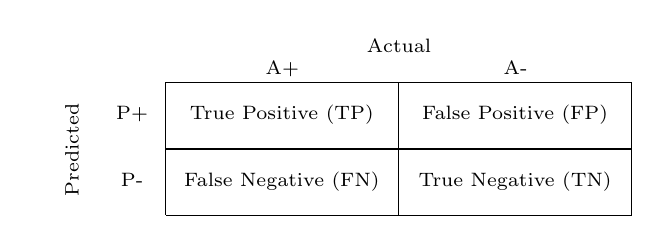
\begin{tikzpicture}[scale=0.4]
      \node at (1,1){
      \scriptsize{
        \begin{tabular}{
            >{\centering}m{1em} >{\centering}m{1em} >{\centering}m{1in} >{\centering\arraybackslash}m{1in}}
          % c>{\centering}m{2em}ccc}
          & & \multicolumn{2}{c}{ Actual}\\
          & & A+ & A- \\
          \cline{3-4}
          & \multicolumn{1}{c|}{} & \multicolumn{1}{c|}{} & \multicolumn{1}{c|}{}\\
          \multirow{3}{*}{\rotatebox[origin=c]{90}{Predicted}}& \multicolumn{1}{c|}{P+} &  \multicolumn{1}{c|}{True Positive (TP)} & \multicolumn{1}{c|}{False Positive (FP)} \\
          &\multicolumn{1}{c|}{}  & \multicolumn{1}{c|}{}& \multicolumn{1}{c|}{} \\
          \cline{3-4}
          & \multicolumn{1}{c|}{} &\multicolumn{1}{c|}{} & \multicolumn{1}{c|}{}\\

          & \multicolumn{1}{c|}{P-} &\multicolumn{1}{c|}{False Negative (FN)}  &\multicolumn{1}{c|}{True Negative (TN)}\\
          & \multicolumn{1}{c|}{} &\multicolumn{1}{c|}{} & \multicolumn{1}{c|}{}\\
          \cline{3-4}
          \end{tabular}
      }};
    \end{tikzpicture}
    \end{center}
\caption{Confusion matrix with truly and falsely positive detected samples (\acs{tp}, \acs{fp}) in the first row, from left to right and the falsely and truly negative detected samples (\acs{fn}, \acs{tn}) in the second row, from left to right.}
\label{fig:CM}
\end{figure}


Experimentation details can be found in Sect.\,\ref{subsec:exp1} to Sect.\,\ref{subsec:exp4} and summarized in Table~\ref{tab:experiment_summary}.
In general terms, all the experiments have been carried out using SERI dataset while \emph{Experiment \#1}(Sect.\,\ref{subsec:exp1}) has been complemented using Duke dataset for comparison purposes. This \emph{Experiment \#1}(Sect.\,\ref{subsec:exp1}) takes from the experimentation reported in \cite{Lemaintre2015miccaiOCT} to evaluate the effects of different feature representations and compares the results to those obtained by Venhuizen\emph{et al.}\,\cite{Venhuizen2015}.
\emph{Experiment \#2 and \#3} (Sect.\,\ref{subsec:exp2}\,\&\,\ref{subsec:exp3})) studies the high-level feature extraction from the volumes using \bow. The former experiments effect of the codebook size in order to find the optimal number of words using a linear classifier; while the later explore more sophisticated classifiers using \added(id = moj){based on} the previously found codebook sizes.
\emph{Experiment \#4} (Sect.\,\ref{subsec:exp4}) accounts for the experimentation using low-level representation.

\begin{landscape}
  \begin{table}[ht]
\caption{The outline and summary of the performed experiments.}
\medskip
\scriptsize{
\begin{center}
\resizebox{1\linewidth}{!}{
\begin{tabular}{l  c	 c  c  c  c  c  c  c }
\toprule
\\
&  Dataset & Pre-processing & Features & Mapping & Representation & Classification & Validation & Evaluation \\
\cmidrule(l){2-9}
\\
\multirow{3}{*}{Common:} & \multirow{3}{*}{SERI} & \multirow{3}{*}{\ac{nlm}} & \ac{lbp},\ac{lbptop} & \multirow{3}{*}{} & \multirow{3}{*}{}  & & \multirow{3}{*}{\ac{lopocv}}& \multirow{3}{*}{} \\
        &      &          & $S = \{8,16,24\}$ & & & & & \\
        &      &          & $R = \{1,2,3\}$  & & & & & \\\\
\midrule
\\
Experiment\#1:  \\
%\hdashline \noalign{\vskip 3pt}
%\\
\multirow{2}{4cm}{Goal: Evaluation of features, mapping and representation} & \multirow{2}{*}{+ Duke} &\multirow{2}{*}{$\sim$} & \multirow{2}{*}{$\sim$} & \emph{gocal} & \ac{bow} & \multirow{2}{*}{\ac{rf}} & \multirow{2}{*}{$\sim$} & \multirow{2}{*}{\ac{se}, \ac{sp}, \cite{Venhuizen2015}}\\
&  & & & \emph{local} & Histogram &  & & \\\\
\midrule
\\
Experiment\#2:\\
%\hdashline \noalign{\vskip 3pt}
%\\
\multirow{2}{4cm}{Goal: Finding the optimum number of words}& \multirow{2}{*}{$\sim$} & + \acs{f} & \multirow{2}{*}{$\sim$} & \emph{global} & \multirow{2}{*}{\ac{bow}} & \multirow{2}{*}{\ac{lr}} & \multirow{2}{*}{$\sim$} & \multirow{2}{*}{ \ac{acc}, \ac{f1}}\\
  & & + \acs{fal} & & \emph{local} & & & & \\\\
\midrule
\\
Experiment\#3: \\
%\hdashline \noalign{\vskip 3pt}
%\\
%\hdashline \noalign{\vskip 3pt}
 \multirow{4}{4cm}{Goal: Evaluation of different pre-processing for high-level features }& \multirow{4}{*}{$\sim$} & \multirow{2}{*}{+\acs{f}} & \multirow{4}{*}{$\sim$} & \multirow{2}{*}{\emph{global}} & \multirow{4}{*}{\ac{bow}} & $3$-\ac{nn} & \multirow{4}{*}{$\sim$} & \multirow{4}{*}{\ac{se}, \ac{sp}}\\
 & & \multirow{2}{*}{+\acs{fal}} & & \multirow{2}{*}{\emph{local}} &  & \ac{rf} & & \\
 & & & & & & \ac{svm} & & \\
 & & & & & & \ac{gb} & & \\
\midrule
\\
Experiment\#4:\\
%\hdashline \noalign{\vskip 3pt}
%\\
%\hdashline \noalign{\vskip 3pt}
\multirow{4}{4cm}{Goal: Evaluation of different pre-processing for low-level features} & \multirow{4}{*}{$\sim$} & \multirow{2}{*}{ +\acs{f}} & \multirow{4}{*}{$\sim$} & \multirow{4}{*}{\emph{global}} & \multirow{4}{*}{Histogram} & $3$-\ac{nn} & \multirow{4}{*}{$\sim$} & \multirow{4}{*}{\ac{se}, \ac{sp}}\\
& & \multirow{2}{*}{+\ac{fal}} & & & & \ac{rf} &  &\\
& & & & & & \ac{svm} & & \\
& & & & & & \ac{gb} & & \\
\\
\bottomrule


\end{tabular}}
\end{center}}
\label{tab:table4}
\end{table}
\end{landscape}


\subsection{SERI-Dataset}\label{sec:exp:dataset:seri}
This data was acquired by Singapore Eye Research Institute (SERI), using CIRRUS TM (Carl Zeiss Meditec, Inc., Dublin, CA) \ac{sdoct} device. The datasets consist of 32 \ac{oct} volumes (16 \ac{dme} and 16 normal cases). Each volume contains 128 B-sane with  dimension of 512 $\times$ 1024 pixels.  All \ac{sdoct} images are read and assessed by trained graders and identifies as normal or \ac{dme} cases based on evaluation of retinal thickening, hard exudates, intraretinal cystoid space formation and subretinal fluid.

\subsection{Duke-Dataset} \label{sec:exp:dataset:duke}
This data published by Srinivasan\,\emph{et al.}~\cite{Srinivasan2014} was acquired in Institutional Review Board-approved protocols using Spectralis \ac{sdoct} (Heidelberg Engineering Inc., Heidelberg, Germany) imaging at Duke University, Harvard University and the University of Michigan. This datasets consist of 45 \ac{oct} volumes (15 \ac{amd}, 15 \ac{dme} and 15 normal). In this study we only consider a subset of the original data containing 15 \ac{dme} and 15 normal \ac{oct} volumes.


\subsection{Experiment \#1}\label{subsec:exp1}

% Experiment structure
%
% Intro:
%   - background
%   - goal / experiment intention / why
%   - data
%   - evaluation
%   - reference to result table
%
% Procedure (by data if more than one):
%   - pre-processing
%   - feature extraction
%   - mapping
%   - feature representation
%   - classifier
%
% Result highlights:
%   - (only a description)

%% Experiment intro
For the completeness of this article, this experiment replicates some of the experiments reported in~\cite{Lemaintre2015miccaiOCT}, using the SERI and Duke datasets.

%% Experiment Procedure
For this experiment, the volumes are pre-processed using \nlm.
\lbp and \lbptop descriptors are detected using the default configuration.
Local and global mapping are used.
Volumes are represented using both low-level and high-level feature extraction. For concordance with~\cite{Lemaintre2015miccaiOCT}, when using \bow the size of the coodebook is fixed to $32$ words.
Finally, the volumes are classified using \ac{rf} classifier with 100 un-pruned trees.

Results are listed in Table~\ref{tab:table1-1}, while the two best performing configurations are compared to Venhuizen\,\textit{et al.}~\cite{Venhuizen2015} in Table~\ref{tab:table1-2}.

%% Experiment Result description
Overall, the obtained results indicate that features driven from \ac{lbp} descriptors are highly discriminative.
Nevertheless, Table~\ref{tab:table1-2} indicates a substantial performance difference between SERI and Duke dataset.
This is attributed to the fact that the volumes in Duke dataset are provided with embedded pre-processing steps.




  \begin{table}[h]
\caption{ Experiment \#1 - Obtained results of classification using SERI and Duke datasets.}% using \ac{rf} with 100 trees. High-level features with \ac{bow} are obtained with $K$ = 32 visual-words.}
\centering
\resizebox{1\linewidth}{!}{

\begin{tabular}{l lr c lr c lr  c  lr c lr c lr}
\toprule
Features & \multicolumn{8}{c}{SERI dataset} & & \multicolumn{8}{c}{Duke dataset}\\
\cmidrule(l){2-9} \cmidrule(l){11-18}
 	& \multicolumn{2}{c}{$\{8,1\}$}& & \multicolumn{2}{c}{$\{16,2\}$}& &\multicolumn{2}{c}{$\{24,3\}$} & & \multicolumn{2}{c}{$\{8,1\}$}& & \multicolumn{2}{c}{$\{16,2\}$}& &\multicolumn{2}{c}{$\{24,3\}$}\\
  \cmidrule(l){2-3}  \cmidrule(l){5-6}  \cmidrule(l){8-9} \cmidrule(l){11-12}  \cmidrule(l){14-15}  \cmidrule(l){17-18}
	       & \ac{se} & \ac{sp} & & \ac{se} & \ac{sp} & &  \ac{se} & \ac{sp} & &  \ac{se} & \ac{sp} & &  \ac{se} & \ac{sp} & &  \ac{se} & \ac{sp} \\
\midrule
  	%\ac{lbp}					& 43.7 & 43.7 & & 37.5 & 50.0 & & 50.00 & 62.50  \\
 	\emph{global}-\ac{lbptop}				       & 56.2 & 62.5 & & \textbf{87.5} & \textbf{75.0} & & 68.7 & 68.7 & & 80.0 & 93.3 & & 73.3 & 86.6 & & 73.3 & 86.6 \\
	%\ac{lbp}+\ac{bow}		& 50.0 & 81.2 & & 57.5 & 68.7 & & 50.0 & 50.0 \\
	\emph{local}-\ac{lbp}	   & \textbf{75.0} & \textbf{87.5} & & 81.2 & 75.0 & & 68.7 & 62.5 & & \textbf{80.0} & \textbf{86.6} & & \textbf{86.7} & \textbf{100} & & 93.3 & 86.6\\
	\emph{local}-\ac{lbptop}   & 62.5 & 68.7 & & 56.2 & 37.5 & & 37.5 & 43.7 & & 80.0 & 86.6 & & 86.6 & 86.6 & & 60.0 & 80.0 \\
\bottomrule
\end{tabular}}
\label{tab:table1-1}
\end{table}






\begin{table}[h]
\caption{Experiment \#1 - Comparing the proposed method by \cite{Venhuizen2015} on SERI and Duke datasets.}% with the \textbf{our two} best proposed methods. $K$ = 32 and \ac{rf} is trained using 100 tress}
\centering
\scriptsize{
\begin{tabular}{l	lr c lr}
\toprule
Data sets 	& \multicolumn{2}{c}{SERI} & & \multicolumn{2}{c}{Duke} \\
  \cmidrule(l){2-3}  \cmidrule(l){5-6}
	         & \ac{se} & \ac{sp} & & \ac{se} & \ac{sp}\\
\midrule
Venhuizen~\textit{et al.} \cite{Venhuizen2015} 		& 61.5 & 58.8 & & 71.4 & 68.7\\
\{\emph{local}-\ac{lbp}\},$\{8,1\}$				   & \textbf{75.0} & \textbf{87.5} & & \textbf{86.6} & \textbf{100.0}   \\
\{\emph{global}-\ac{lbptop}\},$\{16,2\}$				& \textbf{75.0} & \textbf{87.5} & & 80.0 & 86.6  \\


\bottomrule
\end{tabular}}
\label{tab:table1-2}
\end{table}


\subsection{Experiment \#2}\label{subsec:exp2}
% Experiment structure
%
% Intro:
%   - background
%   - goal / experiment intention / why
%   - data
%   - evaluation
%   - reference to result table
%
% Procedure (by data if more than one):
%   - pre-processing
%   - feature extraction
%   - mapping
%   - feature representation
%   - classifier
%
% Remarks (if any)
%
% Result highlights:
%   - (only a description)

%% Experiment intro
In order to determine the optimal size of the codebook when using \bow, this experiment evaluates several codebook sizes on SERI dataset.

%% Experiment procedure
For this experiment, several pre-processing strategies are evaluated: (i) \nlm, (ii) a combination of \nlm and flattening; (iii) a combination of \nlm, flattening and aligning.
\lbp and \lbptop descriptors are detected using the default configuration.
Volumes are represented using the high-level feature extraction by using \bow, where the codebook size has been varied as $k \in \{10, 20, 30, \cdots, 100, 200, \cdots, 500, 1000\}$.
Finally, the volumes are classified using \lr. The choice of a linear classifier avoids that the results get busted by the classifier. In this manner any improvement would be linked to the pre-processing and the size of the codebook.

\begin{landscape}

  \begin{table}
\caption{Experiment \#1 - Optimum number of words for each configuration as a result of \ac{lr} Classification, for high-level feature extraction of \emph{global} and \emph{local}-\ac{lbp}, and \emph{local}-\ac{lbptop} features with different pre-processing. The pre-processing includes: \ac{nf}, \ac{f}, and \ac{fal}.
The achieved performances are indicated in terms of  \acs{acc}, \acs{f1}, \acs{se}, and \acs{sp}}
\centering

\footnotesize{
\resizebox{1\linewidth}{!}{
\begin{tabular}{ll  ccccr	c	ccccr	c ccccr}
\toprule
Features & Pre-processing &    \multicolumn{5}{c}{$\{8,1\}$}  & & \multicolumn{5}{c}{$\{16,2\}$} & & \multicolumn{5}{c}{$\{24,3\}$} \\
  \cmidrule(l){3-7}  \cmidrule(l){9-13}  \cmidrule(l){15-19}
   & &  	\ac{acc}\% & \ac{f1}\% & \ac{se}\% & \ac{sp}\%  & W\# &  & \ac{acc}\% & \ac{f1}\% & \ac{se}\% & \ac{sp}\%  & W\# &  &\ac{acc}\% & \ac{f1}\% & \ac{se}\% & \ac{sp}\%  & W\# \\
\midrule
\\[-2ex]
  	\emph{global}-\ac{lbp}		\\
 	& \acs{nf} & 81.2 &  78.5 & 68.7 &  93.7 & 500 & & 62.5 & 58.0 & 56.2 & 62.5 & 80  & & 62.5  & 62.5 & 62.5 & 62.5 & 80  \\
	& \acs{f}  & 71.9 &  71.0 & 68.7 &  75.0 & 400 & & 68.7 & 66.7 & 62.5 & 75.0 & 300 & & 68.7  & 66.7 & 62.5  & 75.0 & 300	 \\
	& \acs{fal}& 71.9 &  71.0 & 68.7 &  75.0 & 500 & & 71.9 & 71.0 & 68.7 & 75.0 & 200 & & 75.0  & 68.7 & 68.7  & 68.7 & 500	 \\
	%& \acs{fac}& 75.0 & 73.3 & 68.7 &  81.2 & 500 & & 78.1 & 75.8 & 68.7 & 87.5 & 500 & & 68.7  & 68.7 & 68.7  & 68.7 & 90	 \\
	\\
\hdashline \noalign{\vskip 3pt}
\\[-2ex]
 	\emph{local}-\ac{lbp}		\\
 	& \acs{nf}  &\cellcolor[gray]{0.6}75.0  &\cellcolor[gray]{0.6} 75.0 &\cellcolor[gray]{0.6} 75.0  &\cellcolor[gray]{0.6} 75.0 &\cellcolor[gray]{0.6} 70 & & 65.6 & 64.5 & 62.5 & 68.7 & 90 & &  62.5 & 60.0 & 56.2  & 68.7  & 30  \\
	& \acs{f}   & 75.0  & 73.3 & 68.7  & 81.2 & 30 & & 71.8 & 61.0 & 68.7 & 75.0 & 70 & &  62.5 & 62.5 & 62.5  & 62.5  & 100	 \\
	& \acs{fal} & 75.0  & 69.0 & 62.5  & 81.2 & 40 & & 71.9 & 71.0 & 68.7 & 75.0 & 200 & &  68.7 & 66.7 & 68.7 & 62.5 & 10	 \\
	%& \acs{fac}& 68.7 & 68.7 & 68.7 & 68.7 & 300 & & 65.6 & 64.5 & 62.5 & 68.7 & 100 & & 65.6  & 64.5 & 62.5  & 68.7 & 100	 \\
	\\
\hdashline \noalign{\vskip 3pt}
\\[-2ex]
 	\emph{local}-\ac{lbptop}		\\
 	& \acs{nf}	& 68.7 & 68.7 & 68.7 & 68.7 & 400 & & \cellcolor[gray]{0.6}75.0  & \cellcolor[gray]{0.6}75.0   &\cellcolor[gray]{0.6}75.0   &\cellcolor[gray]{0.6}75.0  &\cellcolor[gray]{0.6}500 & & 71.9 & 71.0 & 68.7 & 75.0 & 60	 \\
	& \acs{f}	& 68.7 & 68.7 & 68.7 & 68.7 & 300 & & 68.7  & 66.7   & 62.5   & 75.0  & 50  & & 75.0 & 76.5 & 81.2 & 68.7 & 80	 \\
	& \acs{fal}	& 75.0 & 73.3 & 68.7 & 81.2 & 100 & & 75.0  & 73.3   & 68.7   & 81.2  & 90  & & 75.0 & 69.0 & 62.5 & 81.2 & 70	 \\
	%& \acs{fac}	& 71.9 & 69.0 & 62.5 & 81.2 & 400 & & 75.0  & 73.3   & 68.7   & 81.2  & 100 & & 75.0 & 73.3 & 68.7 & 81.2 & 60	 \\
	\\

\bottomrule
\end{tabular}}}
\label{tab:table2}
\end{table}
\end{landscape}


%\begin{tiny}
  \begin{table}[ht]
\caption{Experiment \#2 - The obtained results, using the optimal number of words in terms of \ac{se} and \ac{sp}.}
\centering

\footnotesize{
\resizebox{1\linewidth}{!}{
\begin{tabular}{ll  lcr	c	lcr	c lcr}
\toprule
Features & Pre-processing &    \multicolumn{3}{c}{$8^{riu2}$}  & & \multicolumn{3}{c}{$16^{riu2}$} & & \multicolumn{3}{c}{$24^{riu2}$} \\
  \cmidrule(l){3-5}  \cmidrule(l){7-9}  \cmidrule(l){11-13}
   & &  	\ac{acc}\% & \ac{f1}\% & W\# &  & \ac{acc}\% & \ac{f1}\% & W\# &  & \ac{acc}\% & \ac{f1}\% & W\#\\
\midrule
  	\emph{global}-\ac{lbp}		\\
 	& \acs{nf} & 68.7 &  93.7 &  500 & & 56.2 & 62.5 & 80  & & 62.5  & 62.5 & 80  \\
	& \acs{f}  & 68.7 &  75.0 &  400 & & 62.5 & 75.0 & 300 & & 62.5  & 75.0 & 300	 \\
	& \acs{fal}& 68.7 &  75.0 &  500 & & 68.7 & 75.0 & 200 & & 68.7  & 68.7 & 500	 \\
	%& \acs{fac}& 68.7   &  81.2 &  500 & & 68.7 & 87.5  & 500 & & 68.7  & 68.7 & 90	 \\
\hdashline \noalign{\vskip 3pt}
 	\emph{local}-\ac{lbp}		\\
 	& \acs{nf} & 75.0  & 75.0 & 70 & & 62.5 & 68.7  & 90 & &  56.2  & 68.7   & 30  \\
	& \acs{f}  & 68.7  & 81.2 & 30 & & 68.7 & 75.0  & 70 & &  62.5  & 62.5 & 100	 \\
	& \acs{fal} & 62.5 & 81.2 & 40 & & 68.7 & 75.0  & 200 & &  68.7 & 62.5 & 10	 \\
	%& \acs{fac}& 68.7 & 68.7 & 300 & & 62.5 & 68.7 & 100 & & 62.5  & 68.7 & 100	 \\
\hdashline \noalign{\vskip 3pt}
 	\emph{local}-\ac{lbptop}		\\
 	& \acs{nf}	& 68.7 & 68.7 & 400 & & 75.0   & 75.0   & 500 & & 68.7 & 75.0 &60	 \\
	& \acs{f}	& 68.7 & 68.7 & 300 & & 62.5   & 75.0 & 50  & & 81.2   & 68.7  & 80	 \\
	& \acs{fal}	& 68.7 & 81.2 & 100 & & 68.7   & 81.2 & 90  & & 62.5   & 81.2 &  70	 \\
	%& \acs{fac}	& 62.5 & 81.2   & 400 & & 68.7   & 81.2 & 100 & & 68.7   & 81.2 &60	 \\

\bottomrule
\end{tabular}}}
\label{tab:table2-2}
\end{table}
%\end{tiny}



The usual construction of the codebook consists of clustering the samples in
the feature space using $k$-means. However, this operation is rather
computationally expensive and convergence of the $k$-means algorithm for all
codebook sizes is not granted.
Nonetheless, Nowak\,\textit{et al.}~\cite{nowak2006sampling} pointed out that randomly generated codebooks can be used at the expenses of accuracy.
Since the goal is to assess the best codebook size not its final performance, for this experiment, the construction of the codebook has been carried out using random initialization $k$-means++ algorithm ~\cite{arthur2007k}, which is usually used as a $k$-means initialization algorithm.

Figure.~\ref{fig:RBOW} shows the \ac{acc} and \ac{f1} score graphs obtained for a single case \footnote{Full set of scores can be found at the github repository} in~\cite{Lemaitre2015}, while the optimal number of words for all the configuration are reported in a compact manner in Table~\ref{tab:table2}.

\added[id=sik]{For the sake of comparison, Table~\ref{tab:table2-2} reports performance of optimal codebook size in terms of \ac{se} and \ac{sp}.}

%% Experiment Result description
In general, the obtained results show, that commonly less number of words is required when higher number of sampling points and radius ($\{S,R\} = \{24,3\}$) is used.
The required number of words decreases for \emph{local}-\ac{lbp} in comparison to \emph{global}-\ac{lbp} as well.
Although it was anticipated that the use of different pre-processing steps affect the optimal number of words, this influence is not substantial and consistent over all the obtained results.


\subsection{Experiment \#3}\label{subsec:exp3}
% Experiment structure
%
% Intro:
%   - background
%   - goal / experiment intention / why
%   - data
%   - evaluation
%   - reference to result table
%
% Procedure (by data if more than one):
%   - pre-processing
%   - feature extraction
%   - mapping
%   - feature representation
%   - classifier
%
% Remarks (if any)
%
% Result highlights:
%   - (only a description)

%% Experiment intro
Once studied the impact of the codebook size in Sect.\,\ref{subsec:exp2}, this experiment explores the improvement associated to use more sophisticated classification strategies.

%% Procedure
For this experiment, several pre-processing strategies are evaluated: (i) \nlm, (ii) a combination of \nlm and flattening; (iii) a combination of \nlm, flattening and aligning.
\lbp and \lbptop features are detected using the default configuration.
Volumes are represented using the high-level feature extraction, \bow. The codebooks are computed using regular $k$-means algorithm which is initialized by $k$-means++, where $k$ is chose accordingly to the findings in \emph{Experiment \#2}.
Finally, the volumes are classified using $k$-\ac{nn}, \ac{rf}, \ac{gb}, and \ac{svm}.

Regarding the classification strategies, $k$-\ac{nn} classifier is trained by considering the 3 nearest neighbor.
The \ac{rf} and \ac{gb} classifier are trained using 100 un-pruned trees, while \ac{svm} classifier is trained with \ac{rbf} kernel.

Table~\ref{tab:table3} shows the obtained results from this experiment, where the best performance are highlighted in \textbf{bold}.

%% Experiment Result description

In general terms, it is observed that \ac{rbf}-\ac{svm} provides the best results and outperforms the others.
This classifier achieve the highest \ac{se} and \ac{sp} of 81.2\% and 93.7\% , respectively using the high-level extraction of \emph{local}-\ac{lbp} descriptor, when the data was preprocessed using \ac{nlm} and \ac{f}.
In general, the classifier achieves the best performance,using the high-level extracted features of \emph{local}-\ac{lbp} and \emph{local}-\ac{lbptop}.
This results are obtained while using a sampling points and radius of $\{S,R\} = \{8,1\}$.

Although the highest results was achieved after additional \ac{f} pre-processing step, the effect of this step in not substantial and consistent through the whole experiment with respect to different classifiers and sampling points.
Moreover, the results indicate that often using the pre-processed data only with \ac{nlm} is sufficient enough.




\subsection{Experiment \#4}\label{subsec:exp4}
% Experiment structure
%
% Intro:
%   - background
%   - goal / experiment intention / why
%   - data
%   - evaluation
%   - reference to result table
%
% Procedure (by data if more than one):
%   - pre-processing
%   - feature extraction
%   - mapping
%   - feature representation
%   - classifier
%
% Remarks (if any)
%
% Result highlights:
%   - (only a description)

%% Experiment intro
This experiment replicates the \emph{Experiment \#3} for the case of low-level extracted features from the volumes.

%% Experiment procedure
For this experiment, several pre-processing strategies are evaluated: (i) \nlm, (ii) a combination of \nlm and flattening; (iii) a combination of \nlm, flattening and aligning.
\lbp and \lbptop descriptors are detected using the default configuration.
Volumes are represented using low-level feature extraction of the \emph{global} mapping.
Finally, the volumes are classified using $k$-\ac{nn}, \ac{rf}, \ac{gb}, and \ac{svm}; using the same configuration of \emph{Experiment \#3}.

The obtained results from this experiment is listed in Table.~\ref{tab:table4}, where the highest results are highlighted in \textbf{bold}.


%% Experiment Result description
The obtained results, shows that \ac{rf} has a better performance while using low-level extracted features, in comparison to the previous experiment where, \ac{svm} had a better performance dealing with high-level extracted features.

The highest results of this experiment, \ac{se} and \ac{sp} of 81.2\% and 81.2\%, respectively, was achieved with \ac{rf} and using \emph{global}-\ac{lbptop} features with sampling points and radius of $\{S,R\}=\{24,3\}$.
In general, in this experiment, \emph{global}-\ac{lbptop} features have better performance in comparison to \emph{global}-\ac{lbp} features and the  classification rates improved while using a higher number of sampling points and radius ($\{S,R\}=\{24,3\}$).

Similar to the previous experiments, although the effects of additional pre-processing steps (\ac{f} and \ac{fal}) is evident for \ac{rf} performance on $\{S,R\} = \{24,3\}$, similar to the previous experiments, this influence is not consistent for all different configurations, in terms of classifier and $\{S,R\}$.


\begin{landscape}

  \begin{table}[ht]
\caption{Experiment \#3 - $k$-\ac{nn} and  \ac{svm} classification with \ac{bow} for the \emph{global} and \emph{local} \ac{lbp} and \emph{local} \ac{lbptop} features with different pre-processing. The optimum number of words were selected based on the previous experiment.}
\centering

\scriptsize{
\resizebox{0.9\linewidth}{!}{
\begin{tabular}{ll  lr	c	lr	c lr c lr	c	lr	c lr}
\toprule
& & \multicolumn{8}{c}{$k$-\ac{nn}} & & \multicolumn{8}{c}{\ac{svm}}\\
\cmidrule(l){3-10} \cmidrule(l){12-19}
Features & Pre-processing &    \multicolumn{2}{c}{$\{8,1\}$}  & & \multicolumn{2}{c}{$\{16,2\}$} & & \multicolumn{2}{c}{$\{24,3\}$}  & &   \multicolumn{2}{c}{$\{8,1\}$}  & & \multicolumn{2}{c}{$\{16,2\}$} & & \multicolumn{2}{c}{$\{24,3\}$} \\
  \cmidrule(l){3-4}  \cmidrule(l){6-7}  \cmidrule(l){9-10}   \cmidrule(l){12-13}  \cmidrule(l){15-16}  \cmidrule(l){18-19}
   & &  	\ac{se}\% & \ac{sp}\% &  & \ac{se}\% & \ac{sp}\% &  & \ac{se}\% & \ac{sp}\%  & & 	\ac{se}\% & \ac{sp}\% &  & \ac{se}\% & \ac{sp}\% &  & \ac{se}\% & \ac{sp}\% \\
\midrule
  	\emph{global}-\ac{lbp}		\\
 	& \acs{nf} & 43.7 &  93.7 &   & 43.7 & 87.5  &  & 43.7  & 62.5  &  & 68.7 & 87.5 & & 62.5 & 62.5 & & 50.0 & 56.2 \\  
	& \acs{f}  & 43.7 &  56.2 &   & 50.0 & 75.0  &  & 62.5  & 56.2  &  & 56.2 & 56.2 & & 56.2 & 75.0 & & 56.2 & 68.7  \\
	& \acs{fa} & 56.2 &  62.5 &   & 43.7 & 81.2  &  & 68.7  & 56.2  &  & 56.2 & 68.7 & & 68.7 & 68.7 & & 56.2 & 75.0	 \\
	%& \acs{fac}& 50   &  75.0 &   & 37.5 & 87.5  &  & 50.0  & 62.5 &  & 50.0 & 75.0 & & 50.0 & 75.0 & & 43.7 & 68.7 \\
\hdashline \noalign{\vskip 3pt}
 	\emph{local}-\ac{lbp}		\\
 	& \acs{nf} & \cellcolor[gray]{0.8}\textbf{75.0} & \cellcolor[gray]{0.8}\textbf{87.5} & & 50.0  & 68.7 &  &  43.7  & 43.7 & & \cellcolor[gray]{0.6}\textbf{75.0} & \cellcolor[gray]{0.6}\textbf{93.7} & & 50.0 & 75.0 & & 56.2 & 56.2    \\
	& \acs{f}  & \cellcolor[gray]{0.8}56.2 & \cellcolor[gray]{0.8}56.2 & & 50.0  & 50.0 &  & 50.0   & 43.7 & &\cellcolor[gray]{0.6}\textbf{81.2} & \cellcolor[gray]{0.6}\textbf{93.7} & & 68.7 & 68.7 & & 68.7 & 75.0 \\
	& \acs{fa} & \cellcolor[gray]{0.8}56.2 & \cellcolor[gray]{0.8}43.7 & & 50.0  & 75.0 &  & 50.0   & 62.5 & & \cellcolor[gray]{0.6}\textbf{75.0} & \cellcolor[gray]{0.6}\textbf{93.7} & & 75.0 & 68.7 & & 68.7 & 68.7  \\
	%& \acs{fac}& 37.5 & 75.0 & & 31.2 & 75.0 &  & 62.5  & 81.2 & & 62.5 & 87.5 & & 56.2 & 43.7 & & 75.0 & 56.2	 \\
\hdashline \noalign{\vskip 3pt}
 	\emph{local}-\ac{lbptop}		\\
 	& \acs{nf} & 56.2 & 75.0 & & 56.2 & 75.0 & & 62.5 & 56.2 & & \cellcolor[gray]{0.8}\textbf{81.2} & \cellcolor[gray]{0.8}\textbf{87.5} & & \cellcolor[gray]{0.8}\textbf{75.0} & \cellcolor[gray]{0.8}\textbf{100} & & 56.2 & 75.0 \\
	& \acs{f} & 62.5 & 43.7 & & 37.5 & 68.7 & & 43.7 & 62.5 & & \cellcolor[gray]{0.8}\textbf{81.2} & \cellcolor[gray]{0.8}\textbf{81.2} & & \cellcolor[gray]{0.8}75.0 & \cellcolor[gray]{0.8}68.7 & & 81.2 & 68.7		 \\
	& \acs{fal}	& 56.2 & 56.2 & & 68.7 & 50.0 & & 43.7 & 62.5 & & \cellcolor[gray]{0.8}62.5 & \cellcolor[gray]{0.8}75.0 & & \cellcolor[gray]{0.8}68.7 & \cellcolor[gray]{0.8}75.0 & & 62.5 & 81.2  \\
	%& \acs{fac} & 43.7 & 68.7 & & 68.7 & 75.0 & & 56.2 & 81.2 & & 56.2 & 87.5 & & 87.5 & 75.0 & & 62.5 & 75.0	 	 \\
\midrule
& & \multicolumn{8}{c}{\ac{rf}} & & \multicolumn{8}{c}{\ac{gb}}\\
\cmidrule(l){3-10} \cmidrule(l){12-19}
Features & Pre-processing &    \multicolumn{2}{c}{$8^{riu2}$}  & & \multicolumn{2}{c}{$16^{riu2}$} & & \multicolumn{2}{c}{$24^{riu2}$}  & &   \multicolumn{2}{c}{$8^{riu2}$}  & & \multicolumn{2}{c}{$16^{riu2}$} & & \multicolumn{2}{c}{$24^{riu2}$} \\
  \cmidrule(l){3-4}  \cmidrule(l){6-7}  \cmidrule(l){9-10}   \cmidrule(l){12-13}  \cmidrule(l){15-16}  \cmidrule(l){18-19}
   & &  	\ac{se}\% & \ac{sp}\% &  & \ac{se}\% & \ac{sp}\% &  & \ac{se}\% & \ac{sp}\%  & & 	\ac{se}\% & \ac{sp}\% &  & \ac{se}\% & \ac{sp}\% &  & \ac{se}\% & \ac{sp}\% \\
\midrule
  	\emph{global}-\ac{lbp}		\\
 	& \acs{nf} & \cellcolor[gray]{0.8}\textbf{68.7} & \cellcolor[gray]{0.8}\textbf{93.7} & & 43.7 & 62.5 & & 50.0 & 68.7  & & 56.2 & 50.0 & & 37.5 & 31.2 & & 50.0 & 43.7\\
	& \acs{f}  & \cellcolor[gray]{0.8}56.2 & \cellcolor[gray]{0.8}50.0 & & 56.2 & 75.0 & & 50.0 & 75.0  & & 50.0 & 56.2 & & 56.2 & 75.0 & & 43.7 & 62.5\\
	& \acs{fa} & \cellcolor[gray]{0.8}68.7 & \cellcolor[gray]{0.8}50.0 & & 56.2 & 62.5 & & 62.5 & 56.2  & & 56.2 & 50.0 & & 68.7 & 50.0 & & 43.7 & 75.0\\
	%& \acs{fac} & 68.7 & 68.7 & & 56.2 & 75.0 & & 50.0 & 68.7& &  50.0 & 68.7 & & 75.0 & 62.5 & & 56.2 & 81.2  \\ 
\hdashline \noalign{\vskip 3pt}
 	\emph{local}-\ac{lbp}		\\
 	& \acs{nf} &  \cellcolor[gray]{0.8}\textbf{81.2} & \cellcolor[gray]{0.8}\textbf{81.2} & & 62.5 & 56.2 & & 56.2 & 56.2 & & 75.0 & 62.5 & & 68.7 & 87.5 & & 50.0 & 75.0   \\
	& \acs{f}  &  \cellcolor[gray]{0.8}56.2 & \cellcolor[gray]{0.8}81.2 & & 62.5 & 68.7 & & 68.7 & 62.5 & & 68.7 & 75.0 & & 50.0 & 75.0 & & 50.0 & 62.5 \\
	& \acs{fa} &  \cellcolor[gray]{0.8}68.7 & \cellcolor[gray]{0.8}62.5 & & 62.6 & 68.7 & & 43.7 & 43.7 & & 56.2 & 50.0 & & 68.7 & 56.2 & & 50.0 & 50.0 \\
	%& \acs{fac}&  62.5 & 68.7 & & 68.7 & 68.7 & & 68.7 & 56.2 & &  56.2 & 50.0 & & 56.2 & 68.7 & & 62.5 & 68.7  \\
\hdashline \noalign{\vskip 3pt}
 	\emph{local}-\ac{lbptop}		\\
 	& \acs{nf} & 68.7 & 62.5 & & \cellcolor[gray]{0.6}\textbf{68.7} & \cellcolor[gray]{0.6}\textbf{81.2} & & 68.7 & 68.7 & & 37.5 & 68.7 & & 62.5 & 81.2 & & 62.5 & 50.0  \\
	& \acs{f} & 50.0 & 62.5 & & \cellcolor[gray]{0.6}62.5 & \cellcolor[gray]{0.6}62.5 & & 43.7 & 75.0 & & 50.0 & 56.2 & & 43.7 & 62.5 & & 50.0 & 62.5		 \\
	& \acs{fal}	& 50.0 & 62.5 & & \cellcolor[gray]{0.6}\textbf{81.2} & \cellcolor[gray]{0.6}\textbf{87.5} & & 50.0 & 68.7 & & 56.2 & 62.5 & & 81.2 & 68.7 & & 75.0 & 68.7  \\
	%& \acs{fac}	 & 56.2 & 81.2 & & 68.2 & 81.2 & & 68.7 & 87.5 & & 75.0 & 68.7 & & 87.5 & 75.0 & & 75.0 & 87.5 	 \\

\bottomrule
\end{tabular}}}
\label{tab:table3}
\end{table}
%\end{tiny}
\end{landscape}

%--------------------------------------------------------
%  \begin{table}[ht]
%\caption{The obtained results of experiment \#2.
%Classification results obtained from low-level representation of global \ac{lbp} and \ac{lbptop} features with different pre-processing.
%Pre-processing steps include: \ac{nf}, \ac{f}, \ac{fal}, and \ac{fac}.
%Different classifiers such as \ac{rf}, \ac{gb}, \ac{svm}, \ac{lr}, and $k$-\ac{nn} are used.
%}
%\medskip
%
%\footnotesize{
%\begin{center}
%\resizebox{1\linewidth}{!}{
%%\begin{tabularx}{1.02\linewidth}{l cc  cc cc c cc cc cc }
%\begin{tabular}{l cc  cc cc c cc cc cc }
%\toprule
%& \multicolumn{6}{c}{\ac{rf}} & &  \multicolumn{6}{c}{\ac{gb}} \\
%\cmidrule(l){2-7} \cmidrule(l){9-14}
%Features &  \multicolumn{2}{c}{$8^{riu2}$}  & \multicolumn{2}{c}{$16^{riu2}$} & \multicolumn{2}{c}{$24^{riu2}$} & &  
%   \multicolumn{2}{c}{$8^{riu2}$}  &  \multicolumn{2}{c}{$16^{riu2}$} & \multicolumn{2}{c}{$24^{riu2}$} \\
%  \cmidrule(l){2-3}  \cmidrule(l){4-5}  \cmidrule(l){6-7} \cmidrule(l){9-10}  \cmidrule(l){11-12}  \cmidrule(l){13-14}
%   &  	\ac{se}\% &  \ac{sp}\%  &  \ac{se}\% &  \ac{sp}\% & 	\ac{se}\% &  \ac{sp}\% & & 
%   \ac{se}\% &  \ac{sp}\% & \ac{se}\% &  \ac{sp}\% & \ac{se}\% &  \ac{sp}\%\\
%\midrule
%  	\emph{global}-\ac{lbp} \\
% 	\acs{nf} & 43.7 & 62.5 &   43.7 & 62.5 & 56.2 & 75   & &  43.7 & 43.7 & 43.7 & 37.5 & 37.5 & 31.25  		\\
%	\acs{f}  & 56.2 & 56.2 &   68.7 & 62.5 & 62.5 & 68.7 & &  25   & 56.2 & 50   & 43.7 & 25   & 43.7 \\
%	\acs{fa} & 65.2 & 56.2 &   50   & 50   & 56.2 & 68.7 & &  43.75& 62.5 & 62.5 & 50   & 31.2 & 31.2 \\
%	\acs{fac}& 56.2 & 62.5 &   56.2 & 62.5 & 68.7 & 56.2 & &  25   & 62.5 & 75   & 81.2 & 93.7 & 87.5\\
%
%\hdashline \noalign{\vskip 3pt}
% 	\emph{global}-\ac{lbptop}		\\
% 	\acs{nf}	 & 56.2 & 68.7 &   68.7  & 87.5 & 68.7  & 81.2 & &  68.7 & 68.7 & 75   & 50   & 56.2 & 43.7\\
%	\acs{f}	 & 56.2 & 62.5 &   81.2  & 68.7 & 81.2  & 81.2 & &  56.2 & 62.5 & 62.5 & 68.7 & 68.7 & 81.2\\
%	\acs{fal}& 68.7 & 62.5 &   75    & 68.7 & 75    & 81.2 & &  56.2 & 43.7 & 62.5 & 62.5 & 75   & 75 \\
%	\acs{fac}& 75   & 68.7 &   75    & 81.2 & 75    & 75   & &  75   & 75   & 75   & 56.2 & 81.2 & 62.5\\
%\midrule
%& \multicolumn{6}{c}{\ac{svm}} & &  \multicolumn{6}{c}{$k$-\ac{nn}} \\
%\cmidrule(l){2-7} \cmidrule(l){9-14}
%Features &  \multicolumn{2}{c}{$8^{riu2}$}  & \multicolumn{2}{c}{$16^{riu2}$} & \multicolumn{2}{c}{$24^{riu2}$} & &  
%   \multicolumn{2}{c}{$8^{riu2}$}  &  \multicolumn{2}{c}{$16^{riu2}$} & \multicolumn{2}{c}{$24^{riu2}$} \\
%  \cmidrule(l){2-3}  \cmidrule(l){4-5}  \cmidrule(l){6-7} \cmidrule(l){9-10}  \cmidrule(l){11-12}  \cmidrule(l){13-14}
%   &  	\ac{se}\% &  \ac{sp}\%  &  \ac{se}\% &  \ac{sp}\% & 	\ac{se}\% &  \ac{sp}\% & & 
%   \ac{se}\% &  \ac{sp}\% & \ac{se}\% &  \ac{sp}\% & \ac{se}\% &  \ac{sp}\%\\
%\midrule
%  	\emph{global}-\ac{lbp}		\\
% 	\acs{nf} & 56.2 & 62.5 & 56.2 & 43.7 & 56.2 & 68.7 & & 37.5 & 50   & 25   & 50   & 37.5 & 68.7 \\
%	\acs{f}  & 75   & 68.7 & 62.5 & 62.5 & 62.5 & 68.7 & & 62.5 & 50   & 56.2 & 75   & 62.5 & 68.7\\
%	\acs{fa} & 75   & 68.7 & 62.5 & 62.5 & 62.5 & 68.7 & & 56.2 & 50   & 56.2 & 75   & 62.5 & 68.7 \\
%	\acs{fac}& 56.2 & 62.5 & 25   & 50   & 43.7 & 62.5 & & 50   & 43.7 & 68.7 & 62.5 & 62.5 & 62.5\\
%
%\hdashline \noalign{\vskip 3pt}
% 	\emph{global}-\ac{lbptop}		\\
% 	\acs{nf}	  & 62.5 & 75   & 62.5 & 93.7 & 56.2 & 87.5 & & 31.2 & 93.7 & 37.5 & 100  & 37.5 & 81.2 \\
%	\acs{f}	  & 68.7 & 75   & 43.7 & 68.7 & 68.7 & 56.2 & & 50   & 56.2 & 56.2 & 75   & 56.2 & 62.5\\
%	\acs{fal} & 68.7 & 62.5 & 62.5 & 56.2 & 56.2 & 68.7 & & 75   & 43.7 & 56.2 & 43.7 & 68.7 & 50  \\
%	\acs{fac} & 68.7 & 68.7 & 68.7 & 87.5 & 68.7 & 87.5 & & 62.5 & 62.5 & 68.7 & 68.7 & 75   & 75\\
%%\midrule
%%
%%& \multicolumn{6}{c}{\ac{lr}} \\
%%\cmidrule(l){2-7} 
%%Features &  \multicolumn{2}{c}{$8^{riu2}$}  & \multicolumn{2}{c}{$16^{riu2}$} & \multicolumn{2}{c}{$24^{riu2}$}  \\
%%  \cmidrule(l){2-3}  \cmidrule(l){4-5}  \cmidrule(l){6-7} 
%%   &  	\ac{se}\% &  \ac{sp}\%  &  \ac{se}\% &  \ac{sp}\% & 	\ac{se}\% &  \ac{sp}\% \\
%%\midrule
%%
%%\emph{global}-\ac{lbp}		\\
%%	\acs{nf}	  & 56.2 & 43.7 & 43.7 & 56.2 & 50 & 68.7\\
%%	\acs{f}	  & 56.2 & 43.7 & 56.2 & 37.5 & 68.7 & 43.7 \\
%%	\acs{fal} & 56.2 & 43.7 & 56.2 & 31.2 & 68.7 & 43.7 \\
%%	\acs{fac} & 62.5 & 56.2 & 56.2 & 62.5 & 56.2 & 56.2\\
%%
%%
%%\hdashline \noalign{\vskip 3pt}
%% 	\emph{global}-\ac{lbptop}		\\
%% 	\acs{nf}  & 50   & 50 &  6 & 93.7 & 0 & 100	\\
%%	\acs{f}	  & 75   & 18 & 50 & 75 & 25 & 81.2\\
%%	\acs{fal} & 93.7 & 6  & 93.7 & 6 & 50 & 43.7\\
%%	\acs{fac} & 50   & 81.2 & 0 & 93.7 & 0 & 100\\
%
%\bottomrule
%
%
%\end{tabular}}
%
%\end{center}}
%\label{tab:table4}
%\end{table}
\begin{landscape}

  \begin{table}[ht]
\caption{Experiment \#3 - Classification results obtained from low-level representation of global \ac{lbp} and \ac{lbptop} features with different pre-processing.
Pre-processing steps include: \ac{nf}, \ac{f}, \ac{fal}.
Different classifiers such as \ac{rf}, \ac{gb}, \ac{svm}, and $k$-\ac{nn} are used.
The most relevant configurations are shaded and the highest results are highlighted in \textbf{bold}.
The configurations which their performances declines with additional pre-processing are shaded in light gray while those with the opposite behavior are shaded with darker gray color.}

\medskip

\scriptsize{
\begin{center}
\resizebox{1\linewidth}{!}{
%\begin{tabularx}{1.02\linewidth}{l cc  cc cc c cc cc cc }
\begin{tabular}{ll cc  cc cc c cc cc cc }
\toprule
&  & \multicolumn{6}{c}{$k$-\ac{nn}} & &  \multicolumn{6}{c}{\ac{svm}} \\
\cmidrule(l){3-8} \cmidrule(l){10-15}
Features & Pre-processing &   \multicolumn{2}{c}{$\{8,1\}$}  & \multicolumn{2}{c}{$\{16,2\}$} & \multicolumn{2}{c}{$\{24,3\}$} & &  
   \multicolumn{2}{c}{$\{8,1\}$}  &  \multicolumn{2}{c}{$\{16,2\}$} & \multicolumn{2}{c}{$\{24,3\}$} \\
  \cmidrule(l){3-4}  \cmidrule(l){5-6}  \cmidrule(l){7-8} \cmidrule(l){10-11}  \cmidrule(l){12-13}  \cmidrule(l){14-15}
   &  & 	\ac{se}\% &  \ac{sp}\%  &  \ac{se}\% &  \ac{sp}\% & 	\ac{se}\% &  \ac{sp}\% & & 
   \ac{se}\% &  \ac{sp}\% & \ac{se}\% &  \ac{sp}\% & \ac{se}\% &  \ac{sp}\%\\
\midrule
  	\emph{global}-\ac{lbp}		\\
 	& \acs{nf} & 37.5 & 50.0   & 25.0 & 50.0   & 37.5 & 68.7 & & 56.2 & 62.5 & 56.2 & 43.7 & 56.2 & 68.7 \\
	& \acs{f}  & 62.5 & 50.0   & 56.2 & 75.0   & 62.5 & 68.7 & & 75.0 & 68.7 & 62.5 & 62.5 & 62.5 & 68.7 \\
	& \acs{fa} & 56.2 & 50.0   & 56.2 & 75.0   & 62.5 & 68.7 & & 75.0 & 68.7 & 62.5 & 62.5 & 62.5 & 68.7 \\
	%\acs{fac}& 50   & 43.7 & 68.7 & 62.5 & 62.5 & 62.5 & & 56.2 & 62.5 & 25   & 50   & 43.7 & 62.5  \\

\hdashline \noalign{\vskip 3pt}
 	\emph{global}-\ac{lbptop}		\\
 	& \acs{nf}	  &  31.2 & 93.7 & 37.5 & 100.0  & 37.5 & 81.2 & &  62.5 & 75.0   & \cellcolor[gray]{0.8}\textbf{62.5} & \cellcolor[gray]{0.8}\textbf{93.7} & 56.2 & 87.5  \\
	& \acs{f}	  &  50.0 & 56.2 & 56.2 & 75.0   & 56.2 & 62.5 & &  68.7 & 75.0   & \cellcolor[gray]{0.8}43.7 & \cellcolor[gray]{0.8}68.7 & 68.7 & 56.2 \\
	& \acs{fal}   &  75.0 & 43.7 & 56.2 & 43.7   & 68.7 & 50.0 & &  68.7 & 62.5   & \cellcolor[gray]{0.8}62.5 & \cellcolor[gray]{0.8}56.2 & 56.2 & 68.7  \\
	%\acs{fac} & 68.7 & 68.7 & 68.7 & 87.5 & 68.7 & 87.5 & & 62.5 & 62.5 & 68.7 & 68.7 & 75   & 75\\	
\midrule	
&  & \multicolumn{6}{c}{\ac{rf}} & &  \multicolumn{6}{c}{\ac{gb}} \\
\cmidrule(l){3-8} \cmidrule(l){10-15}
Features & Pre-processing &   \multicolumn{2}{c}{$8^{riu2}$}  & \multicolumn{2}{c}{$16^{riu2}$} & \multicolumn{2}{c}{$24^{riu2}$} & &  
   \multicolumn{2}{c}{$8^{riu2}$}  &  \multicolumn{2}{c}{$16^{riu2}$} & \multicolumn{2}{c}{$24^{riu2}$} \\
  \cmidrule(l){3-4}  \cmidrule(l){5-6}  \cmidrule(l){7-8} \cmidrule(l){10-11}  \cmidrule(l){12-13}  \cmidrule(l){14-15}
   & &  	\ac{se}\% &  \ac{sp}\%  &  \ac{se}\% &  \ac{sp}\% & 	\ac{se}\% &  \ac{sp}\% & & 
   \ac{se}\% &  \ac{sp}\% & \ac{se}\% &  \ac{sp}\% & \ac{se}\% &  \ac{sp}\%\\
\midrule
  	\emph{global}-\ac{lbp} \\
 	& \acs{nf} & 43.7 & 62.5 &   43.7 & 62.5 & 56.2 & 75   & &  43.7 & 43.7 & 43.7 & 37.5 & 37.5 & 31.25  		\\
	& \acs{f}  & 56.2 & 56.2 &   68.7 & 62.5 & 62.5 & 68.7 & &  25   & 56.2 & 50.0   & 43.7 & 25.0   & 43.7 \\
    & \acs{fal} & 65.2 & 56.2 &   50.0   & 50.0   & 56.2 & 68.7 & &  43.75& 62.5 & 62.5 & 50.0   & 31.2 & 31.2 \\
	%& \acs{fac}& 56.2 & 62.5 &   56.2 & 62.5 & 68.7 & 56.2 & &  25   & 62.5 & 75   & 81.2 & 93.7 & 87.5\\

\hdashline \noalign{\vskip 3pt}
 	\emph{global}-\ac{lbptop}		\\
 	& \acs{nf}	 & 56.2 & 68.7 &   \cellcolor[gray]{0.8}\textbf{68.7}  & \cellcolor[gray]{0.8}\textbf{87.5} & \cellcolor[gray]{0.6}\textbf{68.7}  & \cellcolor[gray]{0.6}\textbf{81.2} & &  68.7 & 68.7 & 75.0   & 50.0   & \cellcolor[gray]{0.8}56.2 & \cellcolor[gray]{0.8}43.7\\
	& \acs{f}	 & 56.2 & 62.5 &   \cellcolor[gray]{0.8}81.2  & \cellcolor[gray]{0.8}68.7 & \cellcolor[gray]{0.6}\textbf{81.2}  & \cellcolor[gray]{0.6}\textbf{81.2} & &  56.2 & 62.5 & 62.5 & 68.7 & \cellcolor[gray]{0.8}68.7 & \cellcolor[gray]{0.8}81.2\\
	& \acs{fal}& 68.7 & 62.5 &   \cellcolor[gray]{0.8}75.0    & \cellcolor[gray]{0.8}68.7 & \cellcolor[gray]{0.6}\textbf{75.0}   & \cellcolor[gray]{0.6}\textbf{81.2} & &  56.2 & 43.7 & 62.5 & 62.5 &\cellcolor[gray]{0.8}\textbf{75.0}   & \cellcolor[gray]{0.8}\textbf{75.0} \\
	%\acs{fac}& 75   & 68.7 &   75    & 81.2 & 75    & 75   & &  75   & 75   & 75   & 56.2 & 81.2 & 62.5\\



%\midrule
%
%& \multicolumn{6}{c}{\ac{lr}} \\
%\cmidrule(l){2-7} 
%Features &  \multicolumn{2}{c}{$8^{riu2}$}  & \multicolumn{2}{c}{$16^{riu2}$} & \multicolumn{2}{c}{$24^{riu2}$}  \\
%  \cmidrule(l){2-3}  \cmidrule(l){4-5}  \cmidrule(l){6-7} 
%   &  	\ac{se}\% &  \ac{sp}\%  &  \ac{se}\% &  \ac{sp}\% & 	\ac{se}\% &  \ac{sp}\% \\
%\midrule
%
%\emph{global}-\ac{lbp}		\\
%	\acs{nf}	  & 56.2 & 43.7 & 43.7 & 56.2 & 50 & 68.7\\
%	\acs{f}	  & 56.2 & 43.7 & 56.2 & 37.5 & 68.7 & 43.7 \\
%	\acs{fal} & 56.2 & 43.7 & 56.2 & 31.2 & 68.7 & 43.7 \\
%	\acs{fac} & 62.5 & 56.2 & 56.2 & 62.5 & 56.2 & 56.2\\
%
%
%\hdashline \noalign{\vskip 3pt}
% 	\emph{global}-\ac{lbptop}		\\
% 	\acs{nf}  & 50   & 50 &  6 & 93.7 & 0 & 100	\\
%	\acs{f}	  & 75   & 18 & 50 & 75 & 25 & 81.2\\
%	\acs{fal} & 93.7 & 6  & 93.7 & 6 & 50 & 43.7\\
%	\acs{fac} & 50   & 81.2 & 0 & 93.7 & 0 & 100\\

\bottomrule


\end{tabular}}
\end{center}}
\label{tab:table4}
\end{table}
\end{landscape}




%%% Local Variables:
%%% mode: latex
%%% TeX-master: "../../main.tex"
%%% End:

%% % include the figures path relative to the master file
% \graphicspath{ {./content/results/figures/} }

% \begin{tikzpicture}
%   \node (t1) [shape=rectangle,draw] {
%     % \begin{table}
%     % \caption{Obtained results using SERI data sets using \ac{rf} with 100 trees. High-level features with \ac{bow} are obtained with $K$ = 32 visual-words.}
%     % \centering
%     \begin{tabular}{lcclcclcccclcclcccclcclc}
%     \toprule
%     Features 	& & &\multicolumn{4}{c}{$8^{riu2}$}&	 & & & &\multicolumn{4}{c}{$16^{riu2}$}& & & & &\multicolumn{4}{c}{$24^{riu2}$} &\\
%       \cmidrule(l){2-8}  \cmidrule(l){10-16}  \cmidrule(l){18-24}
%             & & & SE & & & SP & & & & & SE & & & SP & & & & & SE & & & SP & \\
%     \midrule
%         \ac{lbp}					& & & 43.75 & & & 43.75 & & & & & 37.50 & & & 50.00 & & & & & 50.00 & & & 62.50 & \\
%       \ac{lbptop}				& & & 56.25 & & & 62.50 & & & & & \textbf{87.50} & & & \textbf{75.00} & & & & & 68.75 & & & 68.75 & \\
%       \ac{lbp}+\ac{pca}		& & & 50.00 & & & 62.50 & & & & & 56.25 & & & 37.50 & & & & & 68.75 & & & 68.75 & \\
%       \ac{lbp}+\ac{bow}		& & & 50.00 & & & 81.25 & & & & & 57.50 & & & 68.75 & & & & & 50.00 & & & 50.00 & \\
%       \ac{lbp}+\ac{bow}+\acs{sw}		& & & 75.00 & & & 87.50 & & & & & \textbf{81.25} & & & \textbf{75.00} & & & & & 68.75 & & & 62.5 & \\
%       \ac{lbptop}+\ac{bow}+\acs{sw}		& & & 62.50 & & & 68.75 & & & & & 56.25 & & & 37.50 & & & & & 37.50 & & & 43.75 & \\
%     \bottomrule
%     \end{tabular}
%     % \label{tab:SERI-data}
%     % \end{table}
%     };
% \end{tikzpicture}
% \begin{table}
% \caption{Obtained results using SERI datasets.}% using \ac{rf} with 100 trees. High-level features with \ac{bow} are obtained with $K$ = 32 visual-words.}
% \centering
% \begin{tabular}{lcclcclcccclcclcccclcclc}
% \toprule
% Features 	& & &\multicolumn{4}{c}{$8^{riu2}$}&	 & & & &\multicolumn{4}{c}{$16^{riu2}$}& & & & &\multicolumn{4}{c}{$24^{riu2}$} &\\
%   \cmidrule(l){2-8}  \cmidrule(l){10-16}  \cmidrule(l){18-24}
% 	       & & & SE & & & SP & & & & & SE & & & SP & & & & & SE & & & SP & \\
% \midrule
%   	\ac{lbp}					& & & 43.75 & & & 43.75 & & & & & 37.50 & & & 50.00 & & & & & 50.00 & & & 62.50 & \\
%  	\ac{lbptop}				& & & 56.25 & & & 62.50 & & & & & \textbf{87.50} & & & \textbf{75.00} & & & & & 68.75 & & & 68.75 & \\
% 	\ac{lbp}+\ac{pca}		& & & 50.00 & & & 62.50 & & & & & 56.25 & & & 37.50 & & & & & 68.75 & & & 68.75 & \\
% 	\ac{lbp}+\ac{bow}		& & & 50.00 & & & 81.25 & & & & & 57.50 & & & 68.75 & & & & & 50.00 & & & 50.00 & \\
% 	\ac{lbp}+\ac{bow}+\acs{sw}		& & & 75.00 & & & 87.50 & & & & & \textbf{81.25} & & & \textbf{75.00} & & & & & 68.75 & & & 62.5 & \\
% 	\ac{lbptop}+\ac{bow}+\acs{sw}		& & & 62.50 & & & 68.75 & & & & & 56.25 & & & 37.50 & & & & & 37.50 & & & 43.75 & \\
% \bottomrule
% \end{tabular}
% \label{tab:SERI-data}
% \end{table}

% \begin{tiny}
% \begin{table}
% \caption{Obtained results using Duke datasets.}% using \ac{rf} with 100 trees. High-level features with \ac{bow} are obtained with $K$ = 32 visual-words.}
% \centering
% \begin{tabular}{lcclcclcccclcclcccclcclc}
% \toprule
% Features 	& & &\multicolumn{4}{c}{$8^{riu2}$}&	 & & & &\multicolumn{4}{c}{$16^{riu2}$}& & & & &\multicolumn{4}{c}{$24^{riu2}$} &\\
%   \cmidrule(l){2-8}  \cmidrule(l){10-16}  \cmidrule(l){18-24}
% 	       & & & SE & & & SP & & & & & SE & & & SP & & & & & SE & & & SP & \\
% \midrule
%  	\ac{lbptop}				& & & 80.00& & & 93.33 & & & & & 73.33 & & & 86.67 & & & & & 73.33 & & & 86.67 & \\
% 	\ac{lbp}+\ac{bow}+\acs{sw}		& & & 80.00 & & & 86.67 & & & & & 86.67 & & & 100 & & & & &93.33 & & & 86.67 & \\
% 	\ac{lbptop}+\ac{bow}+\acs{sw}		& & & 80.00 & & & 86.67 & & & & & 86.67 & & & 86.67 & & & & & 60.00 & & & 80.00 & \\
% \bottomrule
% \end{tabular}
% \label{tab:Duke-data}
% \end{table}
% \end{tiny}




%----------

%%% Local Variables:
%%% mode: latex
%%% TeX-master: "../../main.tex"
%%% End:


\section{Conclusions}\label{sec:con}
The work presented here addresses the automatic classification of \ac{sdoct} data to identify subjects with \ac{dme} versus normal.
Based on the reported results, the low level volume 3D features and high level 2D features using patches achieve the most desirable results in the experimental setup presented here.
The comparison against different datasets and methodologies, highlights that:
regardless of using low or high level representations, volume signatures derived from \ac{lbp} texture show high discriminative power for distinguishing \ac{dme} vs normal volumes.

%TOMORROW THE MOON !!


% Our method is based on \ac{lbp} features to describe the texture of \ac{oct} images and we compare different \ac{lbp} features extraction approaches to compute a single signature for the whole \ac{oct} volume.

\vspace{-.2cm}
\bibliography{./content/literature_review}   %>>>> bibliography data in report.bib
\bibliographystyle{splncs03}